
\documentclass[12pt,  % 12 Punkt Schrift
  a4paper,            % DIN A4
  oneside,            % einseitiger Druck
  BCOR=5mm,           % Bindungskorrektur
  parskip=half,       % Halber Abstand zwischen Absätzen
]{scrreprt}
\usepackage{./style/thesisstyle}
\usepackage{enumitem}           % customizations for enumerations
\usepackage{listings}   				% für Codeschnipsel in lstlisting{}

\begin{document}
% !TEX root = ../VPJ.tex
%
% configurations
%

% text field
%-> replace supervisor names with correct ones
\firstSupervisor{Prof. Dr.-Ing. Ulfert Meiners}
\secondSupervisor{}

% text field
%-> replace title with your thesis title
\thesisTitle{Verbundprojekt 2018/2019}
\thesisTitleEN{Verbundprojekt 2018/2019}

%\thesisKind{VPJ}

% text field
%-> replace the key words with your own key words
\keywordsDE{Smart Kamera, Objekterkennung, Farbdetektion, Gehäusekonstruktion, PixyCam, Raspberry Pi}
\keywordsEN{Smart Camera, Objecttracking, Colordetection, Construction, PixyCam, Raspberry Pi}

% text field
%-> replace the text with a description of the thesis
\abstractDE{
Im Rahmen dieser Arbeit werden zwei Kamerasysteme verglichen, welche farbige Objekte auf einem Laufband erkennen und deren Farbe auswerten. Über verschiedene Schnittstellen wird die Auswertung ausgegeben. Dazu werden Anwendungen entworfen, welche die Auswertung auf einem der Systeme ermöglichen. Die Arbeit beschreibt außerdem die konkrete Implementierung des Quellcodes der entworfenen Anwendungen für eines der Kamerasysteme. Ein weiterer zentraler Punkt der Arbeit ist der Entwurf einer geeigneten Halterung für die Kamerasysteme.} 
\abstractEN{
In this thesis, two camera systems are compared, which recognize colored objects on a conveyor belt and evaluate their color. The evaluation is output via various interfaces. For this purpose, applications are designed, which enable the evaluation on one of the systems. The thesis also describes the implementation of the source code of the designed applications for one of the camera systems. Another point of the work is the design of a suitable holder for the camera systems.
} 

% text field
%-> replace jon with your name
\thesisAuthor{Daniel Friedrich}

% text field
%-> enter the submission date
\submissionDate{25. Mai 2019}

% switch - uncomment only one
%-> uncomment NDA or public
%\NDA{yes}
\NDA{no}

% switch - uncomment only one
%-> uncomment the study course you are in
%\studycourse{TI}
%\studycourse{AI}
%\studycourse{WI}
%\studycourse{BMT}
%\studycourse{MAI}
\studycourse{MAA}
    % load all settings
\newcommand{\inlinetodo}[1]{\todo[inline,linecolor=blue,backgroundcolor=blue!25,bordercolor=blue,size=\normalsize]{#1}}

\hyphenation{Ba-che-lor-the-sis Mas-ter-the-sis}

% Cover page here, no page number
% !TEX root = ../VPJ.tex
%
% cover page
% @author Thomas Lehmann
%

\thispagestyle{empty}
\begin{titlepage}
{\fontfamily{phv}\selectfont

% NDA, if needed
% TODO: Select correct font
\begin{textblock*}{\textwidth}(75mm,9mm)
  \begin{minipage}[b][0cm][b]{\textwidth}
  \fontsize{16pt}{16pt}
  \selectfont
    \begin{flushleft}
      \IthesisNDAFull
    \end{flushleft}
  \end{minipage}
\end{textblock*}

% kind of thesis
% TODO: Select correct font
\begin{textblock*}{\textwidth}(30mm,115mm)
  \begin{minipage}[b][0cm][b]{\textwidth}
    \fontsize{22pt}{20pt}
    \selectfont
  	\begin{flushright}
      \IthesisKind
  	\end{flushright}
  \end{minipage}
\end{textblock*}

% author of thesis
% TODO: Select correct font
\begin{textblock*}{\textwidth}(30mm,140mm)
  \begin{minipage}[b][0cm][b]{\textwidth}
  \fontsize{14pt}{20pt}
  \selectfont
    \begin{flushright}
      \IthesisAuthor
  	\end{flushright}
  \end{minipage}
\end{textblock*}

% Title of thesis
% TODO: Select correct font
\begin{textblock*}{\textwidth}(30mm,155mm)
  \begin{minipage}[b][0cm][b]{\textwidth}
  \fontsize{18pt}{20pt}
  \selectfont
  	\begin{flushright}
       \IthesisTitle
  	\end{flushright}
  \end{minipage}
\end{textblock*}

% german version of faculty and department
\begin{textblock*}{\textwidth}(20mm,256mm)
  \begin{minipage}[b][0cm][t]{\textwidth}
  \fontsize{11pt}{10pt}
  \selectfont
    \begin{flushleft}
      \textit{\IthesisFacultyFull} \\
      \textit{\IthesisDepartmentFull}
    \end{flushleft}
  \end{minipage}
\end{textblock*}

% english version of faculty and department
\begin{textblock*}{\textwidth}(52mm,256mm)
  \begin{minipage}[b][0cm][t]{\textwidth}
  \fontsize{11pt}{10pt}
  \selectfont
    \begin{flushright}
      \textit{\IthesisFacultyFullEN} \\
      \textit{\IthesisDepartmentFullEN}
    \end{flushright}
  \end{minipage}
\end{textblock*}
}
\end{titlepage}
\                % this backslash is needed, otherwise LaTeX does wired things ....


% Titlepage is page one even if the number is not shown.
\pagenumbering{roman}
% Title page here
% !TEX root = ../VPJ.tex
%
% title page
% @author Thomas Lehmann
% Hints for titel page and page numbering: https://en.wikipedia.org/wiki/Title_page
%
\newpage
\thispagestyle{empty}
{\fontfamily{phv}\selectfont

  % Author of thesis
  % TODO: Select correct font
  \vspace*{1cm}
  \begin{minipage}[b]{\textwidth}
    \fontsize{14pt}{20pt}
    \selectfont
    \begin{center}
      \IthesisAuthor
    \end{center}
  \end{minipage}

  % Title of thesis
  % TODO: Select correct font  
  \vspace{1.5cm}
  \begin{minipage}[b][0cm][b]{\textwidth}
    \fontsize{18pt}{20pt}
    \selectfont
    \begin{center}
      \IthesisTitle  	  
  	\end{center}
  \end{minipage}

  % Important information
  % TODO: Select correct font  
  \begin{textblock*}{\textwidth}(40mm,210mm)
    \begin{minipage}[b]{\textwidth}
      \fontfamily{ptm}\selectfont
      \fontsize{12pt}{14pt}
      \selectfont
      \IthesisKindDE ~eingereicht im Rahmen der \IthesisExaminationDE \\

      im Studiengang \IstudyCourseName \\
      am \IthesisDepartmentFull \\
      der Fakultät Technik und Informatik\\
      der Hochschule für Angewandte Wissenschaften Hamburg\\

      Betreuender Prüfer: \IfirstSv \\

      Eingereicht am: \ISubDate \\
    \end{minipage}
  \end{textblock*}
}


% Abstract page here
% !TEX root = ../VPJ.tex
%
% abstract page
% @author Thomas Lehmann
%
\newpage
\thispagestyle{empty}   % TODO: This page should show page number
\clearpage
\textbf{\IthesisAuthor}

\vspace{0.5cm}
\textbf{Thema der Arbeit}

\IthesisTitle

\vspace{0.3cm}
\textbf{Stichworte}

\IkeyWordsDE

\vspace{0.3cm}
\textbf{Kurzzusammenfassung}

\begin{minipage}{\textwidth}
\IabstractDE
\end{minipage}

\vspace{1.0cm}
\textbf{\IthesisAuthor}

\vspace{0.3cm}
\textbf{Title of Thesis}

\IthesisTitleEN

\vspace{0.3cm}
\textbf{Keywords}

\begin{minipage}{\textwidth}
\IkeyWordsEN
\end{minipage}

\vspace{0.3cm}
\textbf{Abstract}

\IabstractEN


% Table of contents here
\tableofcontents

% path to the chapters folder is set to find the images used there
\graphicspath{ {./chapters/} }

\setcitestyle{square}

% Chapters
\clearpage
\pagenumbering{arabic}
\chapter{Einleitung}\label{kap:Einleitung}
Im Verbundprojekt Autonome Systeme soll ein Fertigungsprozess mit autonom agierenden Robotern automatisiert werden. Dazu befinden sich acht Stationen mit jeweils zwei Arbeitsplätzen und einem Platz zum Lesen oder Schreiben von RFID-Tags im Versuchsaufbau. Station 1 repräsentiert dabei das Rohteillager und Station 8 das Fertigteillager. Die Arbeitsschritte werden durch Aufenthalt der Werkstücke für eine bestimmte Zeit an den Arbeitsplätzen simuliert. Je nach Produkt, das hergestellt werden soll, variiert die Anzahl, Reihenfolge, und Bearbeitungszeit der Stationen. Zum Transport der Werkstücke zwischen den Stationen werden autonom agierende Roboter mit einer Greifzange eingesetzt. Die Navigation der Roboter wird mit Hilfe von ermittelten Positionsdaten realisiert, die mit Kameras ermittelt werden. Als Software wird, für die Programmierung der Roboter, Matlab/Simulink eingesetzt. Für die Auftragsplanung wird Qt verwendet. Das Speichern der Produktionsdaten erfolgt über eine MySQL-Datenbank und die RFID-Technologie wird mit CODESYS angesteuert.

\section{Aufgaben Gewerk 1}

Das Gewerk 1 ist zuständig für:

\begin{itemize}
    \item die Fertigungsplanung,
    \item die Visualisierung des Fertigungsprozesses,
    \item das Beschreiben und Auslesen der RFID-Tags auf den Werkstücken und
    \item das Ablegen aller produktionsrelevanten Daten in der MySQL-Datenbank.
\end{itemize}

Die Fertigungsplanung soll die über das visuelle HMI eingegebenen Aufträge verwalten und den Robotern ihre Aufträge zuweisen. Die Visualisierung soll die Roboter und ihre Position so wie die Arbeitsstationen darstellen. Über die Visualisierung soll ebenfalls die Auftragseingabe stattfinden und der aktuelle Fortschritt eines Auftrags abgebildet werden. Ebenso ist die vom Fertigungsrechner mit Hilfe der RFID-Technologie durchgeführte Verfolgung der Werkstücke darzustellen.

Der Fertigungsrechner soll die RFID-Tags der Werkstücke mit Hilfe der RFID-Schreib-Lese-Köpfe beschreiben, beziehungsweise auslesen, um so eine Verfolgung der Werkstücke durch den Produktionsprozess zu ermöglichen. Auf dem Fertigungsrechner befindet sich auch der Server für die MySQL-Datenbank, die alle produktionsrelevanten Daten speichert und sowohl vom Programm für die RFID-Technologie, als auch von der Fertigungsplanung lesend und schreibend angesprochen wird.

\section{Gesamtkonzept Gewerk 1}

Das Gesamtkonzept von Gewerk 1 ist in Abbildung \ref{fig:Gesamtkonzept} dargestellt.

\begin{figure}[htb]
	    \centering
	    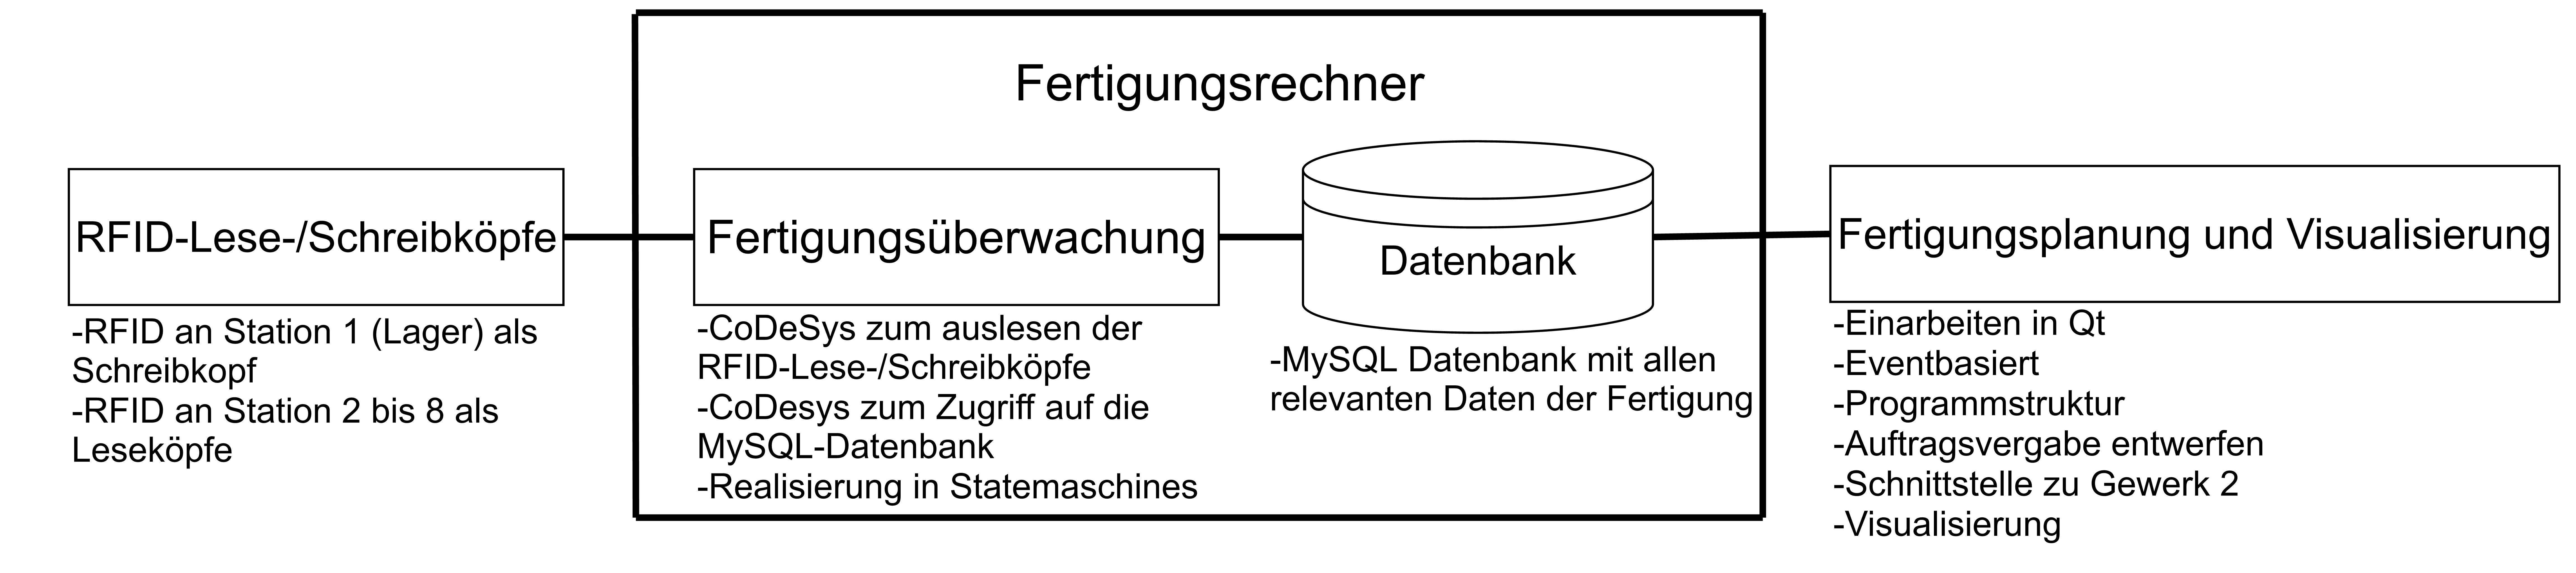
\includegraphics[width=1\linewidth]{Bilder/Konzept2.png}
        \caption{Gesamtkonzept von Gewerk 1}
        \label{fig:Gesamtkonzept}
\end{figure}

Die Fertigungsplanung und die Visualisierung werden in einem gemeinsamen Programm, dass mit Qt geschrieben wurde, realisiert. Die Fertigungsplanung empfängt für die Visualisierung über Ethernet per UDP/IP die Daten des Navigationsrechners. Die Kommunikation mit den Robotern wird ebenso von der Fertigungsplanung über WLAN per UDP/IP realisiert. Die Kommunikation zur Datenbank, die sich auf dem Fertigungsrechner befindet, findet über Ethernet statt. Die RFID-Schreib-Lese-Köpfe werden über ein Interface mittels Profibus-DP an den Fertigungsrechner angeschlossen. Das Programm zum Auslesen, beziehungsweise Beschreiben, der RFID-Tags wird mit CODESYS geschrieben und läuft auf einer Soft-SPS auf dem Fertigungsrechner. An Station 1 werden die RFID-Tags des Werkstücks beschrieben und an den Stationen 2 bis 8 ausgelesen. Über SQL4Automation kann das Programm auf die Datenbank lesend und schreibend zugreifen. In der Datenbank sind alle für den Produktionsprozess relevanten Daten abgelegt. Es handelt sich um eine relationale MySQL-Datenbank. Die Datenbank dient auch zur Kommunikation zwischen dem CODESYS-Programm auf dem Fertigungsrechner und der Fertigungsplanung. 


%\input{chapters/Vorhandenes_System}
%\input{chapters/PixyCam}
%\input{chapters/Marktrecherche}
% !TEX root = ../VPJ.tex

\chapter{Grundlagen und Konzepte von Qt}
\label{sec:Grundlagen}

In diesem Kapitel werden einige Grundlagen erläutert, die zum Verständnis der späteren Kapitel der Arbeit beitragen. 

Qt ist eine plattformübergreifende Anwendungsentwicklungsumgebung für Desktop\-anwendungen, eingebettete und mobile Systeme. Unterstützt werden unter anderem Linux, OS X,  Windows, Android, iOS, BlackBerry oder Sailfish OS. 

Die Umgebung ist in C++ geschrieben, weshalb vorwiegend in dieser Sprache programmiert wird. Eine Besonderheit an Qt ist die Benutzung eines Signal-Slot-Systems. 

Ähnlich anderen Entwicklungsumgebungen bietet Qt mit einem implementierten Designer, Möglichkeiten zur GUI-Programmierung mit vorgefertigten Widgets (vgl. \cite{qt_allgemein}).

Die nächsten Abschnitte zeigen einige Besonderheiten von Qt und Konzepte, die in der Ausarbeitung des Projekts verwendet wurden. 

\section{Eventbasiertes System}
\label{sec:Eventbasiert}

Innerhalb von Qt werden Signale und Slots zur Kommunikation zwischen Objekten genutzt. Das Signal-Slot Konzept ersetzt das in anderen Umgebungen verwendete Callback-System, welches beispielsweise in Eclipse bei der Java-Programmierung oder in Visual Studio mit C\# verwendet wird. 

\begin{figure}[htb]
    \centering
    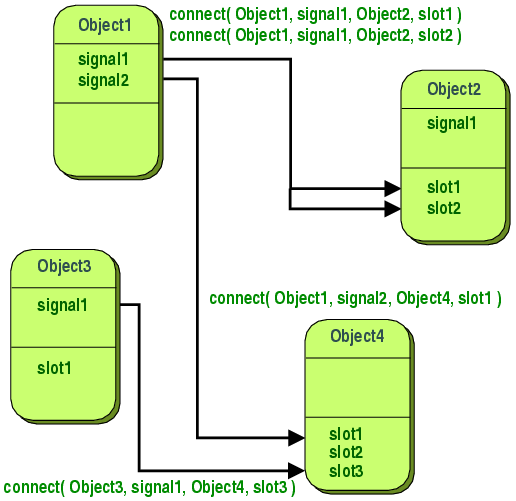
\includegraphics[width=0.5\textwidth]{Abbildungen/signalslots.png}
    \caption[Signale und Slots in Qt \newline Quelle: \textit{https://doc.qt.io/qt-5/signalsandslots.html}]{Signale und Slots in Qt}		
    \label{fig:signalslots}
\end{figure}

In Abbildung \ref{fig:signalslots} ist das Konzept visuell dargestellt. Ein Signal wird immer dann emittiert, wenn ein bestimmtes Event auftritt. Die in Qt verwendeten Widgets stellen bereits viele dieser Signale bereit, können jedoch um Eigene ergänzt werden. 

Das Gegenstück zu den Signalen sind Slots, welche als Antwort auf ein Signal aufgerufen werden. Es können beliebig viele Signale an einen Slot gebunden werden. Es ist ebenfalls möglich Signale direkt an weitere Signale zu binden. 

Ein Slot kann wie eine normale Funktion auch mittels Funktionsaufruf verwendet werden.  

Nähere Informationen zu diesem Konzept, zu Signalen und zu Slots können der Quelle \cite{qt_signalslot} entnommen werden. 

Um Signale und Slots zu verbinden werden verschiedene Möglichkeiten bereitgestellt. In dieser Arbeit wurde hauptsächlich mit der connect() Funktion gearbeitet, die von jeder Klasse, die von QObject erbt, bereitgestellt wird. 

\begin{lstlisting}[frame=single, breaklines=true, numbers=left, stepnumber=2, firstnumber=1, numberstyle = \tiny, caption=Connect Signals and Slots ,label=lst:Connect]
QObject::connect(const QObject *sender, const char *signal, const QObject *receiver, const char *method, Qt::ConnectionType type = Qt::AutoConnection)
\end{lstlisting}

In Listing \ref{lst:Connect} ist der Connect-Aufruf vollständig dargestellt. Hinzuzufügen ist, dass der letzte Übergabeparameter, ConnectionType, optional ist, da er als Standardwert QT::AutoConnection beinhaltet. Die ersten beiden Parameter enthalten also immer die Senderseite, die letzten beiden Parameter die Empfängerseite. Dabei ist zuerst das Objekt anzugeben, welches sendet oder empfängt und danach das Signal, bzw. der Slot, der genutzt werden soll. 

\section{Sockets}
\label{sec:QTSocket}

Die Kommunikation über UDP wird in Qt mit einem QUdpSocket bereitgestellt. Der Socket bietet Funktionen, mit denen UDP-Datagramme gesendet und empfangen werden können. 

Um einen Datenaustausch zu ermöglichen wird der Socket mittels einer Bind()-Methode an eine spezielle Adresse und einen Port gebunden. Vorteil dieser Implementierung ist, dass beim Erhalt einer Nachricht ein readyRead()-Signal emittiert wird, auf das sich verbunden werden kann. 

Sobald das readyRead()-Signal emittiert wurde, liefert hasPendingDatagrams() true zurück. Das Datagramm kann anschließend über readDatagram() oder receiveDatagram() ausgelesen werden (vgl. \cite{qt_socket}).

Außerdem unterstützt die Klasse UDP multicast.

Wenn ein Datagramm nicht ausgelesen wird, wird kein weiteres readyRead()-Signal emittiert, bis dieses ausgelesen wurde. 

\section{Datenbank in Qt}
\label{sec:QTDatabase}

Um möglichst einfach Datenbanken in Qt zu implementieren, wird die Klasse QSqlDatabase (vgl. \cite{qt_database}) bereitgestellt. Diese Klasse ist für die Verbindung und Kommunikation an eine bestehende Datenbank zuständig. Der Datenbanktyp wird über den eingeladenen Treiber bestimmt. In dieser Arbeit sollte auf eine Datenbank vom Typ MYSQL zugegriffen werden.

Um den Treiber der Entwicklungsumgebung von Qt bekannt zu machen war es notwendig eine MYSQL Library einzubinden. Dies konnte gelöst werden, indem die Datei "`MySQLLib.dll"', welche zum Beispiel im MySQL Connector zu finden ist (Pfad: C:\textbackslash Program Files\textbackslash MySQL\textbackslash MySQL Connector.C 6.1\textbackslash lib), an einen Ort kopiert wird, dessen Pfad von der Entwicklungsumgebung erkannt wird. Ein Möglicher Ort ist C:\textbackslash Windows. 

Nachdem sich mit dem Setzten von Nutzername, Passwort, Datenbankname und Host auf die Datenbank verbunden wurde, können die gegebenen Funktionen verwendet werden. 

In dieser Arbeit wurde eine QSqlQuery innerhalb der QSqlDatabase verwendet, um die Daten der Datenbank auszulesen und zu manipulieren. Die Query stellt Funktionen zur Verfügung, mit denen die gängigen SELECT, INSERT und UPDATE Befehle umgesetzt werden können.  

\section{State Machines in Qt}
\label{sec:StateMachines}

Um entwickelte Zustandsautomaten zu implementieren, bietet Qt ein Konzept "`State Machines"' mit dazugehörigen Klassen. 

Dieses Konzept basiert darauf, einen, in beispielsweise UML vorliegenden, Zustandsgrafen möglichst einfach zu implementieren. 

Eine einfache Zustandsmaschine, dargestellt in Abbildung \ref{fig:StateMachineexample}, kann wie folgt implementiert werden:

\begin{figure}[htb]
    \centering
    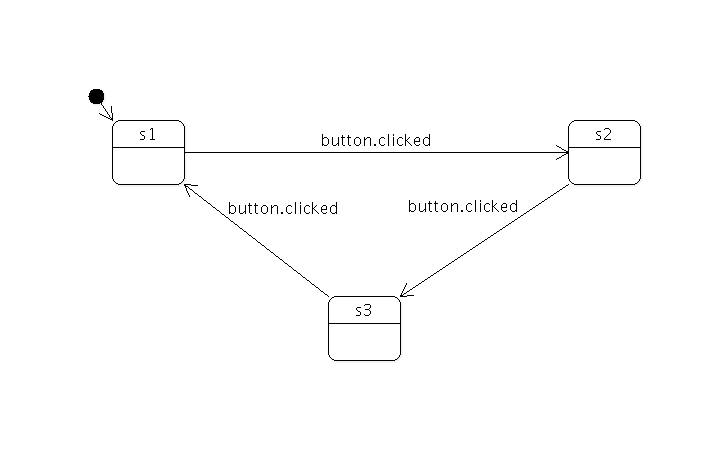
\includegraphics[width=0.7\textwidth]{Abbildungen/statemachinebutton.png}
    \caption[State Machine Beispiel \newline Quelle: \textit{https://doc.qt.io/qt-5/statemachine-api.html}]{State Machine Beispiel}		
    \label{fig:StateMachineexample}
\end{figure}

Zunächst wird die State Machine und ihre Zustände erzeugt (Listing \ref{lst:SM1}). 

\begin{lstlisting}[frame=single, breaklines=true, numbers=left, stepnumber=2, firstnumber=1, numberstyle = \tiny, caption=State Machine Beispiel Teil 1 ,label=lst:SM1]
    QStateMachine machine;
    QState *s1 = new QState();
    QState *s2 = new QState();
    QState *s3 = new QState();
\end{lstlisting}

Anschließend werden jedem Zustand alle für diesen Zustand vorhandenen Transitionen mit der QState::addTransition() Funktion hinzugefügt (Listing \ref{lst:SM2}). Dabei wird angegeben, bei welchem Event (Signal) die Transition ausgeführt werden soll. Wenn ein Transitionssignal außerhalb des Zustands auftritt, wird die Transition nicht ausgeführt. 

\begin{lstlisting}[frame=single, breaklines=true, numbers=left, stepnumber=2, firstnumber=1, numberstyle = \tiny, caption=State Machine Beispiel Teil 2 ,label=lst:SM2]
    s1->addTransition(button, SIGNAL(clicked()), s2);
    s2->addTransition(button, SIGNAL(clicked()), s3);
    s3->addTransition(button, SIGNAL(clicked()), s1);
\end{lstlisting}

Listing \ref{lst:SM3} zeigt, wie anschließend die Zustände dem Zustandsautomaten hinzugefügt werden. Außerdem wird der initiale Zustand gesetzt, der bei Programmstart aktiv sein soll. 

\begin{lstlisting}[frame=single, breaklines=true, numbers=left, stepnumber=2, firstnumber=1, numberstyle = \tiny, caption=State Machine Beispiel Teil 3 ,label=lst:SM3]
    machine.addState(s1);
    machine.addState(s2);
    machine.addState(s3);
    machine.setInitialState(s1);
\end{lstlisting}

Abschließend muss die Zustandsmaschine gestartet werden (Listing \ref{lst:SM4}). Ab diesem Zeitpunkt reagiert der Automat auf die Transitionen und wechselt zwischen den Zuständen. 

\begin{lstlisting}[frame=single, breaklines=true, numbers=left, stepnumber=2, firstnumber=1, numberstyle = \tiny, caption=State Machine Beispiel Teil 4 ,label=lst:SM4]
    machine.start();
\end{lstlisting}

Hauptvorteil der so implementierten Zustandsmaschine ist, dass diese vollkommen asynchron zum restlichen Programm abläuft. Somit müssen keine zusätzlichen Schleifen in Tasks gestartet werden. 

Um Funktionen mit einem Zustand zu verknüpfen kann ein Signal, welches jeder Zustand emittiert, genutzt werden. Bei dem Eingang in einen Zustand wird das Signal entered() emittiert, bei dem Verlassen eines Zustands das Signal exited(). In dieser Arbeit wurde ausschließlich mit dem entered() Signal gearbeitet, da dies die Anforderungen ausreichend erfüllt hat. 

Das aufgezeigte Beispiel und weitergehende Erklärungen zu State Machines und den weiteren Klassen sind in \cite{qt_statemachine} zu finden. Darunter sind auch Konzepte zu finden, die ermöglichen, Eigenschaften direkt an einen Zustand zu binden. 

\section{QListWidget}
\label{sec:QListWidgetItem}

Das QListWidget ermöglicht es, selbst programmierte QListWidgetItems in einer Liste zu organisieren und darzustellen. Zusätzlich werden diverse Funktionen bereitgestellt, mit denen sich die QListWidgetItems ordnen, ergänzen oder finden lassen (vgl. \cite{qt_listwidget}). 

Über die Auswahl der allgemeinen Widgets kann das QListWidget im Layout-Manager ausgewählt werden. 

% !TEX root = ../VPJ.tex

\chapter{Aufgabenstellung}
\label{sec:Aufgabenstellung}

Um an
%\input{chapters/Umsetzung}
%\input{chapters/Abgeleitete_Anforderungen}
% !TEX root = ../VPJ.tex

\chapter{Schnittstellen}
\label{sec:Schnittstellen}

Schnittstellen

\section{Kommunikation zu Gewerk 2}


\label{sec:Gewerk2Protokoll}

Robotererrortypen beschreiben

\subsection{Sequenzdiagramm}
\label{sec:sequenzdiagram}

\inlinetodo{Sequenzdiagramm Kommunikation}
\inlinetodo{Telegram Gewerk 2}

\subsection{Fehlertypen und Behebung}
\label{sec:Error}

\subsubsection{Fehlertyp 1}
\subsubsection{Fehlertyp 2}
\subsubsection{Fehlertyp 3}

% !TEX root = ../VPJ.tex

\chapter{Implementierung}
\label{sec:Implementierung}

Implementierung

\section{Programmstruktur}

\begin{figure}[htb]
    \centering
    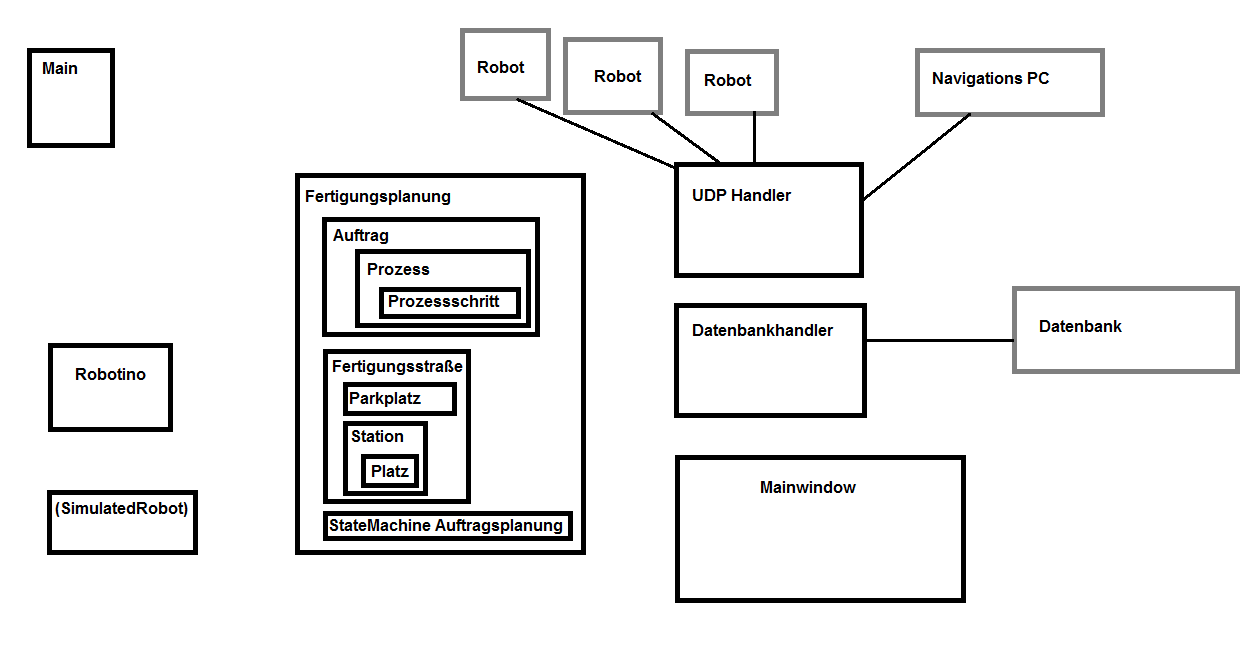
\includegraphics[width=0.9\textwidth]{Abbildungen/Klassendiagramm.PNG}
    \caption{Klassendiagramm}		
    \label{fig:Klassendiagramm}
\end{figure}



\section{Databasehandler}
\section{UDP-Handler} 
\label{sec:UdpHandler}
\section{Robotino} 



\section{Auftrag, Prozess, Prozessschritt} 
\label{sec:AuftragProzessSchritt}

Die im Programm auftretenden Aufträge sind in einer bestimmten Struktur organisiert. Diese variiert zu der in der Datenbank abgespeicherten Struktur. So wird über die Visualisierung ein Auftrag angelegt. Jeder so angelegte Auftrag beinhaltet ein oder mehrere Prozesse. In der Datenbank sind dies komplementär gesehen die Werkstücke. Jeder Prozess besteht aus mehreren Prozessschritten, die den genauen Ablauf eines Prozesses beschreiben. 

Auftrag, Prozess und Prozessschritt sind in verschiedene Klassen geschrieben. Folgend werden diese Klassen näher beleuchtet. 

\subsection{Prozessschritt}
\label{sec:Prozessschritt}

Ein Prozessschritt besteht aus genau einer Stations-ID verknüpft mit einer festen Bearbeitungsdauer in Sekunden. Dies beschreibt für einen Teil eines Prozesses. In einer Fortschritts-Flag wird festgehalten, ob der Prozessschritt bereits bearbeitet wurde, oder noch bearbeitet werden muss. 

Der Prozessfortschritt kann ein Signal emittieren, welches anzeigt, dass sich der Fortschritt geändert hat.

\subsection{Prozess}
\label{sec:Prozess}

Ein Prozess, in der Datenbank Werkstück, beinhaltet eine Liste von Prozessschritten. Diese Liste bestimmt mit ihrer Reihenfolge und Länge die Bearbeitungsvorschrift für ein Werkstück. Jeder Prozess besitzt zudem einen Fortschritt, eine eindeutige ID und eine ReferenzID. 

Mit der eindeutigen ID kann später ein Prozess innerhalb des Programms wiedergefunden werden. Nur die in Aufträgen befindlichen Prozesse erhalten eine aufsteigende laufende Nummer als eindeutige ID. Die in der Initialisierung erzeugten Prozesse oder die über die Visualisierung erzeugten Prozesse (folgend Referenzprozesse) erhalten keine spezielle eindeutige ID, sondern eine aufsteigende eindeutige ReferenzID. Dies führt dazu, nicht alle Informationen in den einzelnen Prozessen halten zu müssen, sondern auf den initialisierten Referenzprozess zugreifen zu können. 

Die ReferenzID eines Prozesses einhält die eindeutige ID des zugehörigen Referenzprozesses. 

Zur Prozesskontrolle gibt es zusätzlich noch verschiedene Flags die den Status des Prozesses widerspiegeln. Dazu gehört ein Blocked- und ein InProgress-Flag. Das InProgress-Flag wird gesetzt, sobald ein Werkstück an einer Station bearbeitet wird. Das Blocked-Flag kann über die Hard-Code Area (vgl. Kapitel \ref{sec:HardCode}) gesetzt werden und verhindert eine weitere Bearbeitung. 

Jeder Prozess enthält einen Timer, der die verbrauchte Zeit an einem Arbeitsplatz kontrolliert. Der Timer wird gestartet, sobald ein Werkstück an einer Station bearbeitet wird, die nötige Zeit wird dem zugehörigen Prozessschritt entnommen. Bei Ablauf des Timers wird die Funktion TimerElapsed() aufgerufen, in der der zugehörige Prozessschrittfortschritt auf fertig gesetzt und das InProgress-Flag zurückgesetzt wird. 

Über die beiden Signale ProzessFinished und FortschrittUpdated kann bekannt gemacht werden, dass sich ein Fortschritt eines Prozesses geändert hat oder die Arbeit an einer Station beendet wurde und das Werkstück bereit ist für Abholung.

Mit der im Prozess enthaltenen Funktion UpdateFortschritt() wird der Fortschritt eines Prozesses anhand der beinhalteten Prozessschritte aktualisiert. Dazu wird die Prozessschrittliste durchgegangen und für jeden Prozessschritt, der als fertig markiert wurde ein entsprechender Fortschritt zum Prozessfortschritt addiert. Die einzelnen Prozessschritte sind dabei so gewichtet, dass die Summe aus allen Prozessschritten, wenn alle abgeschlossen sind, 100 ergibt. Durch Rundungsfehler können in der aktuellen Umsetzung nicht mehr als 25 Prozessschritte je Prozess sauber dargestellt werden. Sollten mehr Prozessschritte erforderlich sein, so müsste die Fortschrittsberechnung angepasst werden.

\begin{figure}[htb]
    \centering
    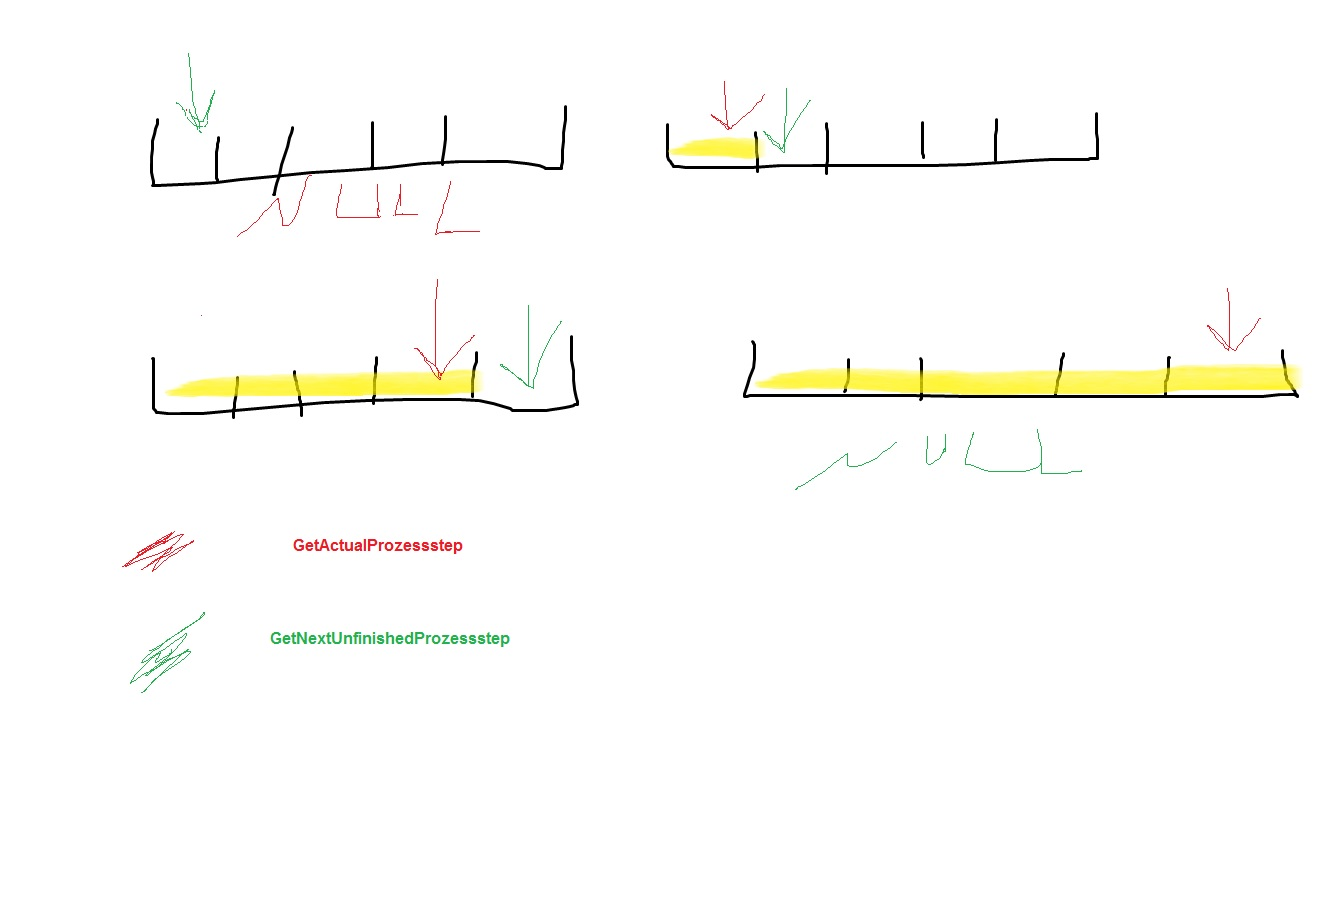
\includegraphics[width=0.9\textwidth]{Abbildungen/GetProzessstep.PNG}
    \caption{Visualisierung des Rückgabewertes der Funktionen GetNextUnfinishedProzessstep() und GetActualProzessstep()}		
    \label{fig:GetProzessstepFunktionen}
\end{figure}

Um auf den richtigen Prozessschritt innerhalb der Liste zuzugreifen sind zwei unterschiedliche Funktionen implementiert. Beide Funktionen unterscheiden sich ausschließlich in ihrem Rückgabewert. In Abbildung \ref{fig:GetProzessstepFunktionen} sind alle möglichen Fälle Prozessschrittliste leer oben links, ein oder mehrere Prozessschritte in der Liste oben rechts und unten links und Liste voll unten rechts dargestellt. Dabei ist zu erkennen, dass die Funktion GetNextUnfinishedProzessstep() immer den nächsten Prozessschritt zurückliefert, der noch nicht bearbeitet wurde. Bei voller Liste wird NULL zurückgegeben. Anders hierzu die Funktion GetActualProzessstep(), die NULL bei leerer Liste zurückgibt und sonst den letzten fertigen Prozessschritt. 

Die Funktion GetActualProzessstep() wird in der Fertigungsplanung zur Planung der Aufträge verwendet (siehe \ref{sec:CheckAuftrag}). GetNextUnfinishedProzessstep() findet Anwendung sobald auf einem aktuellen Prozess eine Änderung auftritt oder umgesetzt werden soll. Wenn beispielsweise der Timer abgelaufen ist, wird in der Funktion TimerElapsed() über der zurückgegebene Prozessschritt als fertig markiert.

\subsection{Auftrag}
\label{sec:Auftrag}

Die Klasse Auftrag enthält eine Liste von Prozessen und darin enthaltenen Prozessschritten und bündelt somit alle drei Klassen. Ähnlich dem Prozess gibt es einen Fortschritt, der sich anteilig aus den einzelnen Prozessfortschritten errechnet und eine eindeutige ID mit derer der Auftrag wiedergefunden und verwaltet werden kann. 

Mit dem Signal FortschrittUpdated kann bekannt gemacht werden, dass sich der Fortschritt geändert hat und z.B. die Visualisierung aktualisiert werden. Das Signal wird gesendet, sobald die Funktion UpdateFortschritt() aufgerufen wurde. In dieser Funktion werden alle enthaltenen Prozesse auf ihren Fortschritt überprüft und im Auftrag gegebenenfalls angepasst. Die Fertigungsplanung verknüpft Auftrag, Prozess und Prozessschritt derartig, dass ein Fortschrittsupdate innerhalb eines Prozessschrittes eine Aktualisierung des Prozessfortschritt hervorruft. Dies wiederum lässt den entsprechenden Auftragsfortschritt aktualisieren (siehe Listing \ref{lst:Auftragserzeugung}).

Ein bestimmter Prozess aus der Liste kann über die Funktion GetProzessByID() mit seiner eindeutige ID zurückgegeben werden. 

Weiterhin werden zwei Funktionen bereitgestellt, die von der Fertigungsplanung genutzt werden um Prozesse oder Prozessschritte zu erhalten. Die Funktion GetNextUnfinishedProzesssteps() gibt, mit Hilfe der Funktion GetNextUnfinishedProzessstep() aus dem Prozess, eine Liste aller entsprechenden Prozessschritte zurück (vgl. Abschnitt \ref{sec:Prozess}). Über die Funktion GetAllUnfinishedProzesses() werden alle Prozesse zurückgegeben, die noch unfertige Prozessschritte enthalten, sofern diese nicht blockiert sind. Hiermit werden in der Fertigungsplanung die zu bearbeitenden Prozesse ausgewählt (siehe \ref{sec:CheckAuftrag}).

\section{Fertigungsplanung}
\label{sec:Fertigungsplanung}

Die Klasse Fertigungsplanung enthält alle verfügbaren Roboter, die Datenbankschnittstelle, die abzuarbeitenden Aufträge (vgl. Abschnitt \ref{sec:AuftragProzessSchritt}), die Fertigungsstraße und eine State Machine zur Verteilung von Roboteraufträgen. Außerdem wird auf Events reagiert, die von der Visualisierung oder anderen Quellen kommen. Zu den Events gehören Statusänderungen des Roboters, hinzufügen von Aufträgen oder Prozessen und Funktionen, die über die Hard-Code Area (vgl. Kapitel \ref{sec:HardCode}) angestoßen werden können. 
In der Fertigungsplanungsklasse werden somit alle Funktionalitäten gebündelt, die nicht direkt mit der Visualisierung zusammenhängen. 

\subsection{Initialisierung}
\label{sec:Fertigunginit}

Um die Fertigungsplanung zu initialisieren wird zunächst in der Funktion InitProzesses() ein Grundzustand hergestellt, in der mindestens 5 Prozesse vorhanden sind. Dazu werden zunächst über einen Datenbankaufruf alle dort verfügbaren Prozesse in eine Liste geschrieben. 

Sollte die Liste weniger als 5 Elemente beinhalten, also in der Datenbank zu Programmstart weniger als 5 Prozesse vorhanden sein, so werden 5 neue zuvor definierte Prozesse (Abschnitt \ref{sec:Standardprozesse}) angelegt und die Liste so überschrieben. 

Die erzeugten Prozesse werden abschließend in die Datenbank geschrieben. Außerdem erhalten alle Prozesse gemäß ihrer Schritte und Dauer in der Visualisierung einen entsprechenden Tooltip (vgl. Kapitel \ref{sec:tooltips}). 

Die Prozessliste kann über die Funktion AddProzess() dynamisch während das Programm läuft erweitert werden. Dies geschieht bei absenden eines eingestelltes Prozesses in der Visualisierung (\ref{sec:Prozesseingabe}). 

\subsubsection{Aufträge hinzufügen}

Durch Einstellen und Absenden eines Auftrags in der Visualisierung (\ref{sec:Auftragseingabe}) wird die Funktion AddAuftrag() aufgerufen. In dieser Funktion wird zunächst ein leeres Auftragsobjekt erzeugt und diesem die nächst höhere Auftragsnummer aus der Datenbank zugeordnet.  

Für jeden Prozesseintrag aus der Visualisierung wird nun die angegebene Anzahl des jeweiligen Prozesses eine Prozesskopie erzeugt. Den so kopierten Prozessen werden alle zugehörigen Prozessschritte als Kopie angehängt, um eigenständige Aufträge zu erhalten. Zuletzt werden die Prozesse und Aufträge miteinander verknüpft (siehe Listing \ref{lst:Auftragserzeugung}).

\begin{lstlisting}[frame=single, breaklines=true, numbers=left, stepnumber=2, firstnumber=1, numberstyle = \tiny, caption=Auftragserzeugung und Verknüpfungen,label=lst:Auftragserzeugung]
Auftrag *A = new Auftrag();

for (int prozesscounter = 0; prozesscounter < 5; prozesscounter++) //5 Prozess UI Elemente
{
    for (int i = 0; i < Avalues[prozesscounter]; i++) //Anzahl der eingegebenen Prozesszahl
    {
        Prozess *p = new Prozess();
        [...]  // Prozess + Prozessschritte kopieren
        A->Prozesse.append(p);
        QObject::connect(p, &Prozess::FortschrittUpdated, A, &Auftrag::UpdateFortschritt);
        QObject::connect(p, &Prozess::ProzessFinished, this, &Fertigungsplanung::StationReady);
    }
}
\end{lstlisting}

Abschließend wird der Auftrag der Auftragsliste angehängt, an die Datenbank gesendet und ein Auftragsitem in der Visualisierung erzeugt (Kapitel \ref{sec:Auftragsuebersicht}). 

\subsubsection{Standardprozesse}
\label{sec:Standardprozesse}

Folgend werden die in Abschnitt \ref{sec:Fertigunginit} erwähnten Standardprozesse näher beleuchtet. 

Um ein möglichst ausgeglichenes Fertigungsbild zu schaffen wurden die fünf Standardprozesse so untereinander abgestimmt, dass diese unterschiedlichen Kriterien genügen. 

Zunächst wurde darauf geachtet, dass die Prozesse unterschiedlich viele Prozessschritte beinhalten. Abbildung \ref{fig:Fahrweganalyse} kann entnommen werden, dass die Prozesse zwischen zwei und sechs einzelne Prozessschritte erfordern. In der Abbildung ist weiterhin dargestellt, welche Station als Start und Ziel je Prozessschritt angefahren wird. 

\begin{figure}[htb]
    \centering
    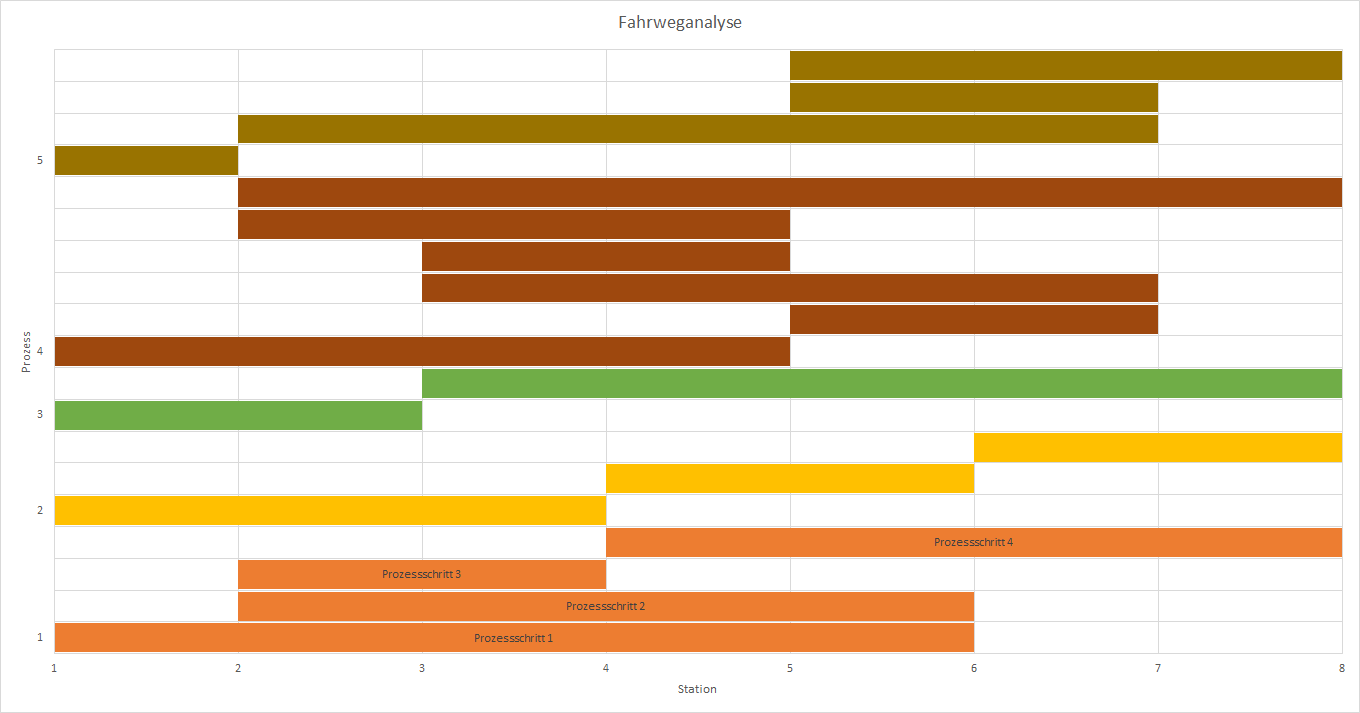
\includegraphics[width=0.9\textwidth]{Abbildungen/Fahrweganalyse.PNG}
    \caption{Diagramm Fahrweganalyse}		
    \label{fig:Fahrweganalyse}
\end{figure}

Zu erkennen ist, dass jeder Prozess bei Station 1 beginnt und in Station 8 endet. Die Einzelnen Prozesse (siehe farbliche Unterscheidung) sind dabei von unten nach oben zu lesen, beginnend mit Prozessschritt 1. 

Aus dem Diagramm können weiterhin potentielle Kollisionsherde und "`Staugefahren"' erkannt werden. Die Standardprozesse wurde so angepasst, dass alle Stationen möglichst gleichmäßig häufig durchfahren werden. Weiterhin kann aus dem Diagramm abgelesen werden, ob durch ungünstige Auftragsplanung ein Deadlock angefahren werden kann, also alle Aufträge irgendwann durch andere Aufträge blockiert sein können. Da keine Schleifen zwischen den Stationen entstanden sind kann gewährleistet werden, dass alle Aufträge in jeder Belegung nach einiger Zeit abgearbeitet werden können, wenn die Werkstücke in Station 8 entnommen werden.

Das Diagramm in Abbildung \ref{fig:Stationsanalyse} zeigt eine genauere Analyse der Stationen. Angenommen wird, dass jeder der Standardprozesse genau ein mal abgearbeitet wird. Auf der linken y-Achse, die zu den bunten Säulen gehört, ist die Belegungsdauer jeder Station in Sekunden angegeben. Die rechte, den hellgelben Säulen zugeordnete y-Achse bezeichnet die Anzahl der Anfahrten an eine Station. 

\begin{figure}[htb]
    \centering
    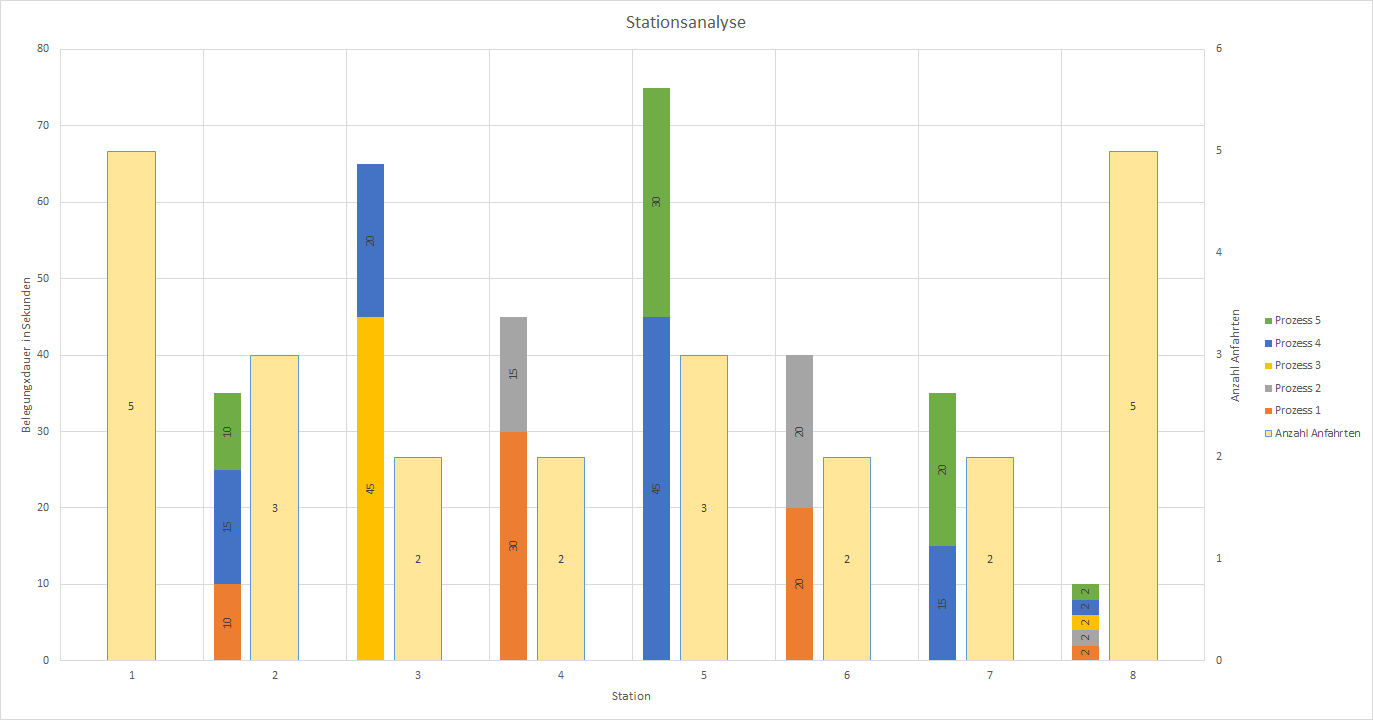
\includegraphics[width=0.9\textwidth]{Abbildungen/Stationsanalyse.PNG}
    \caption{Diagramm Stationsanalyse}		
    \label{fig:Stationsanalyse}
\end{figure}

Es ist zu erkennen, dass Station 1 und 8 genau fünf mal angefahren werden, also je Prozess ein mal. Die weiteren Stationen 2 bis 7 werden zwei- bis dreimal angefahren. So wird sichergestellt, dass die Stationen möglichst gleichmäßig belastet werden. 

Die farblich unterschiedlichen Säulen zeigen die kürzeste Belegungsdauer der Arbeitsplätze an. Die Balken ergeben sich durch die Dauer eines einzelnen Prozessschrittes an einem Arbeitsplatz. Es  Belegungsdauer für alle Prozesse zwischen 35 und 75 Sekunden je Station liegt. Die 2 Sekunden Bearbeitungsdauer je Prozess an Station 8 sind dabei vernachlässigt worden und gewährleisten nur ein sicheres Herausnehmen der Werkstücke durch den Menschen, ohne dass sich der Roboter noch im Entladezyklus befindet. 

Als Besonderheit ist an Station 5 zu erkennen, dass es drei Anfahrten, aber nur zwei verschiedene Prozesse gibt. Dies liegt darin begründet, dass Prozess 4 Station 5 zwei mal anfährt mit verschieden langen Zeiten. Dadurch ist die Gesamtzeit in Station 5 auch am höchsten, gehört jedoch zu großen Anteilen zum selben Prozess. Station 2 hat die kürzesten Bearbeitungszeiten je Prozess, da diese Station von drei verschiedenen Prozessen angefahren wird. Gegensätzlich dazu ist die Bearbeitungszeit an Station 23 von Prozess 3 mit 45 Sekunden sehr hoch angesetzt, da dieser Prozess keine weitere Station anfährt. 

Es wurde versucht, die durchschnittliche Belegungsdauer der Stationen anzugleichen, um alle Arbeitsplätze möglichst homogen auszulasten. Zu erkennen ist, dass die minimale

Als Nebeneffekt ergibt sich, dass die Roboter möglichst ausgeglichen über die gesamte Fertigungsstraße fahren und die Gefahr von Staus oder Kollisionen dadurch verringert wird. 

\subsection{Roboter Statusänderungen}

Wenn eine der in der Fertigungsplanung enthalten Roboterklassen ein Event feuert, welches eine Statusänderung beinhaltet (vgl. Kapitel \ref{sec:UdpHandler}), wird über Funktionen in der Fertigungsplanung auf diese reagiert. So wird der Greifer oder das Statusflag eines Roboters bei einer Änderung aktualisiert. Beim Empfanges eines Errorevents des Roboter wird je nach Errortyp eine Meldung ausgegeben und individuell auf die Robotererror reagiert. 

Weiterhin wird durch Ablauf des Timers eines Arbeitsplatzes dieser in der Fertigungsstraße aktualisiert und auf bereit geschaltet. 


\subsubsection{Roboterstatus geändert}

Bei Änderung des Roboterstatus wird die Funktion OnRobotStatusChanged() aufgerufen. Dabei wird zunächst der aufrufende Roboter ausgewählt und zwischengespeichert. Sollte sich der Status des Roboter auf eins geändert haben, also der Roboter auf dem Weg zu etwas ist, so wird unterschieden ob sich der Roboter auf einem Parkplatz oder einem Arbeitsplatz befunden hat.

Von einem Parkplatz (auch Ladestation) kommend wird dieser in der Datenbank und der Visualisierung wieder freigegeben. Wenn der Roboter zuletzt an einer Station war, so wird diese jetzt für andere Roboter freigegeben und der Roboter wird in der Datenbank aus dem Arbeitsplatz gelöscht. 

\subsubsection{Greiferstatus geändert}

Die Prozessaktualisierungen basieren auf der Änderung des Greifers des Roboters. Es wird vorausgesetzt, dass sich der Greifer zu keinem Zeitpunkt willkürlich öffnet oder schließt, sondern nur bei Aufnahme oder Abgabe eines Werkstücks an einer Station. 

Das Schließen des Greifers eines Roboters bedeutet somit immer, dass ein Werkstück aufgenommen wurde. Somit wird in der Datenbank der Arbeitsplatz, an dem sich der Roboter befindet freigegeben und kann für andere Aufträge genutzt werden. Der Arbeitsplatz wird in der Visualisierung und der Datenbank freigegeben. Zuletzt wird der Tooltip des Arbeitsplatzes (vgl. Kapitel \ref{sec:tooltips}) auf einen leeren String gesetzt. 

Beim Öffnen des Greifers wird ein Werkstück in einen Arbeitsplatz einer Station gelegt. Daraufhin wird die Zuordnung des Werkstücks zu dem entsprechenden Roboter gelöscht. Mit der Werkstücks-ID kann nun aus der Auftragsliste der zugehörige Prozess identifiziert werden. Der Timer des so gefundenen Prozesses wird jetzt gestartet, somit läuft die Bearbeitung des Werkstücks an dem Arbeitsplatz. In der Visualisierung und Datenbank wird der Arbeitsplatz von reserviert auf belegt aktualisiert.

Weiterhin wird das Werkstück, dass dem Roboter zu diesem Zeitpunkt zugeordnet ist an der Station an der sich der Roboter zuletzt aufgehalten hat gelöscht und der zugehörige Arbeitsplatz wird freigegeben. 

\subsubsection{Roboter Error geändert}

Bei Auftreten eines Errors im Roboter wird je nach Typ eine Error-Meldung ins Log geschrieben. 

Die Error-Meldungen des Roboters wurden bewusst nicht automatisiert behandelt, da dem Benutzer die Kontrolle über das Gesamtsystem behalten sollte. Somit muss je nach Fehlertyp eine unterschiedlicher Lösungsweg verfolgt werden. 

Die auftretenden Fehler und der Lösungsweg ist in Kapitel \ref{sec:Error} zu finden. 

\subsection{Hard-Code Funktionen}

Die mit der Hard-Code Area erzeugten Befehle aus der Visualisierung (vgl. Kapitel \ref{sec:HardCode}) werden in verschiedenen Funktionen verarbeitet. So wird beispielsweise der Parkplatz oder eine Station in Datenbank und Visualisierung freigegeben, ein Roboter defekt geschaltet oder ein Arbeitsplatz als defekt markiert oder repariert. 

\subsection{Zustandsdiagramm}

Das Zustandsdiagramm in Abbildung \ref{fig:Auftragsplanung} beschreibt die Logik der Auftragsvergabe an die Roboter. Das Diagramm wurde anschließend als State Machine (vgl. \ref{sec:StateMachines}) implementiert. 

\begin{figure}[htb]
    \centering
    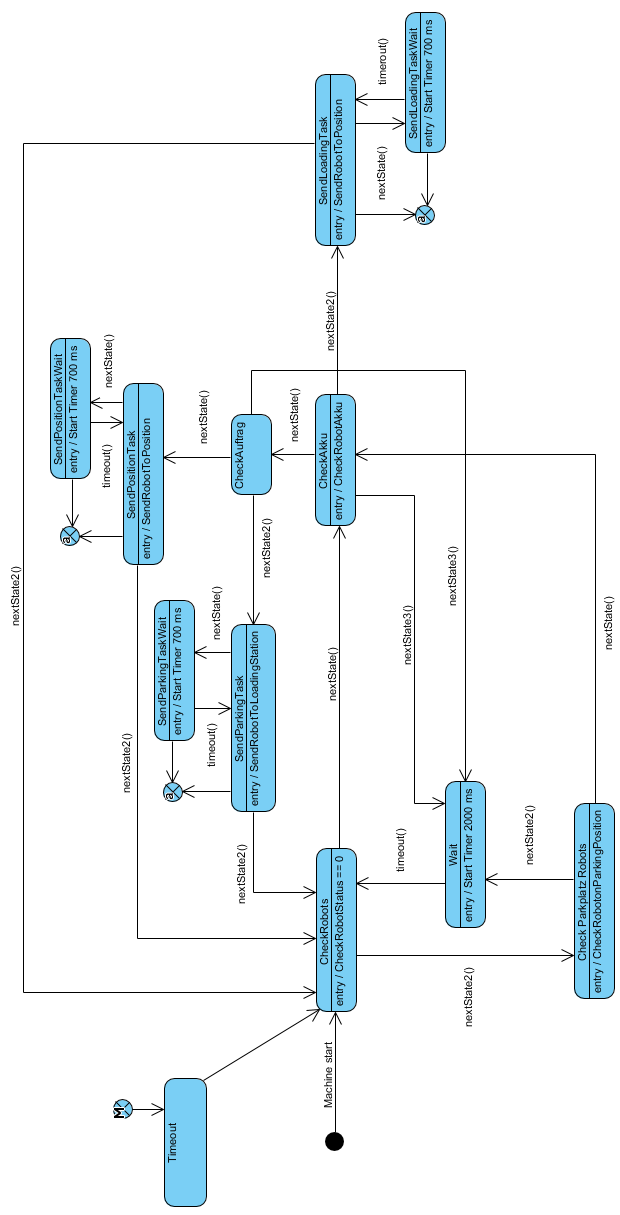
\includegraphics[width=0.8\textwidth]{Abbildungen/Auftragsplanung_rotated.PNG}
    \caption{Zustandsdiagramm der Auftragsplanung}		
    \label{fig:Auftragsplanung}
\end{figure}

In der Abbildung sind die Zustände mit Namen dargestellt. Alle Zustände haben eine komplementäre Funktion, die nach einem Zustandswechsel als Entry-Action aufgerufen wird. Eine genaue Funktionsbeschreibung der Zustände ist in Kapitel \ref{sec:StateMachineImplementierung} zu finden. Um zwischen den Zuständen zu wechseln werden die mit Pfeilen eingezeichneten Transitionen verwendet. Die Pfeilbeschriftung beinhaltet dabei das Signal, welches für den Zustandswechsel genutzt wird. Um das Diagramm übersichtlich zu gestalten, wurden die Timeout-Transitionen nicht vollständig eingezeichnet, sondern enden in einem kreisförmigen Xa-Zustand. Dieser führt direkt zu dem XM-Zustand oben links und leitet in den Zustand Timeout weiter. 

\subsection{State Machine Implementierung}
\label{sec:StateMachineImplementierung}

Im Quellcode werden zunächst alle Zustände erzeugt und der State Machine hinzugefügt. Anschließend werden alle Transitionen zwischen den Zuständen erzeugt und der State Machine hinzugefügt. Hierbei werden definierte Signale genutzt, die zuvor in der Header Datei deklariert wurden. In der Main-Funktion werden abschließend die Zustände mit den entsprechenden zugehörigen Funktionen verknüpft (vgl. \ref{sec:Main}). 

Um die State Machine zu starten wird, nachdem der Initialzustand bekannt gemacht wurde, die Start-Funktion aufgerufen. Eine verkürzte Darstellung der Aufrufe ist in Listing \ref{lst:StartStateMachine} abgebildet. 

\begin{lstlisting}[frame=single, breaklines=true, numbers=left, stepnumber=2, firstnumber=1, numberstyle = \tiny, caption=Start und Initialisierung der State Machine,label=lst:StartStateMachine]
    QStateMachine StateMachine;
    QState *StateCheckRobots = new QState;

    StateMachine.addState(StateCheckRobots);
    StateCheckRobots->addTransition(this, SIGNAL(nextState()), StateCheckAkku);

    StateMachine.setInitialState(StateCheckRobots);
    StateMachine.start();

    QObject::connect(StateCheckRobots, &QState::entered, this, &Fertigungsplanung::CheckRobots);
\end{lstlisting}

\subsubsection{Zustand CheckRobots}

Im Initialzustand der State Machine, CheckRobots, werden alle vier Roboter nacheinander auf Bereitschaft überprüft. Die Reihenfolge der zu überprüfenden Roboter wird dabei durch einen hierfür entwickelten Shuffle-Algorithmus (\ref{sec:shuffle}) bestimmt. 

Ein Roboter gilt als bereit, wenn er als Status 0 zurückgibt, nicht als defekt markiert ist und als lebend gilt. Sobald ein geprüfter Roboter alle drei Kriterien erfüllt wird dieser ausgewählt und in den weiteren Zuständen, gefolgt von CheckAkku, genutzt. Die anderen Roboter werden bis zum nächsten Aufruf des Zustands CheckRobots vernachlässigt.

Sollte keiner der vier Roboter alle drei Kriterien erfüllen wird in den Zustand CheckParkplatzRobots gewechselt.

\subsubsection{Zustand CheckParkplatzRobots}

Wie im Zustand CheckRobots werden alle vier Roboter anhand von Kriterien auf Bereitschaft überprüft. Dazu wird ebenfalls die Reihenfolge zufällig bestimmt.

Anstatt den Roboterstatus wie beim Zustand CheckRobots auf 0 zu prüfen, wird ein Status zwischen 201 und 204 erwartet. Diese vier Stati repräsentieren die vier Parkplätze auf denen sich ein Roboter befinden kann. 

Durch die Aufteilung der Zustände CheckRobots und CheckParkplatzRobots erfolgt eine Priorisierung der Roboter, die sich bereits in den Stationen befinden und einen Auftrag fertig abgearbeitet haben. Nur wenn kein Roboter in den Stationen verfügbar ist wird auf die auf den Parkplatz befindlichen Roboter zurückgegriffen. Dadurch werden Situationen vermindert, in denen sich die Roboter bei der Stationsarbeit gegenseitig behindern.

Sollte keiner der auf den Parkplatz befindlichen Roboter alle weiteren Kriterien erfüllen wird in den Zustand Wait gewechselt.

\subsubsection{Zustand Wait}

Da in Qt aufgrund der eventbasierten Programmierung (vgl. \ref{sec:Eventbasiert}) keine Endlosschleifen vorgesehen sind wurde im Zustand "`Wait"' mittels Timer die Zustandsmaschine künstlich verlangsamt. Ein Entfernen des Zustands führt zum Programmabsturz, da in kürzester Zeit die interne Eventliste voll geschrieben wird. Auf externe Events wie Mauseingaben oder Ereignisse vom Betriebssystem könnte somit nicht mehr reagiert werden. 

Durch den Zustand Wait können andere Programmevents und Ereignisse des Betriebssystems abgearbeitet werden, während 2000 ms auf das timeout()-Signal des Timers gewartet wird. 

Nach Ablauf des Timers wird in den Initialzustand CheckRobots gewechselt.

\subsubsection{Zustand CheckAkku}

Der Zustand CheckAkku gewährleistet einen Tiefentenladungsschutz der Roboter. Sobald ein Roboter in den ersten beiden Zuständen ausgewählt wurde wird überprüft, ob sein Akkustand größer gleich 25 Prozent ist. Es wird davon ausgegangen, dass kein Auftrag plus eine Fahrt zum Laden mehr als 25 Prozent Akku verbraucht. Der Wert wurde empirisch ermittelt. 

Sollte der Akkustand unter 25 Prozent liegen, wird der Roboter über Zustand SendLoadingTask zu einer freien Ladestation geschickt. Wenn keine Ladestation frei ist wird in den Zustand Wait gewechselt. 
Bei einem Akkustand von über 25 Prozent wird der Zustand CheckAuftrag aufgerufen. 

\subsubsection{Zustände SendLoadingTask, SendParkingTask, SendPositionTask}

Um bei Kommunikation mit den Robotern in den Zuständen SendLoadingTask, SendPositionTask und SendParkingTask sicherzustellen, dass die Nachricht empfangen wurde, wird diese mehrfach gesendet, bis die Übertragung erfolgreich war (siehe Kapitel \ref{sec:sequenzdiagram}). Es wird nach jedem Sendevorgang ein kurzer Wartezustand aufgerufen, der, gleich dem Zustand Wait, einen Programmabsturz verhindert. Mit dem individuellen Wartezustand kann ebenfalls das bei aktuell 700 ms angesetzte Sendeintervall eingestellt werden. 

Aus allen den drei Send......Task Zuständen und ihren zugehörigen Wartezuständen kann über ein Ablauf eines Timers in den Zustand Timeout gewechselt werden. Der Timer wird beim erstmaligen Eintritt in einen der Zustände Send......Task gestartet und läuft nach 25 Sekunden ab. Dieser Timer gewährt eine Absturzsicherheit des Programms bei Roboterausfall oder anderweitigem Fehlschlagen der Kommunikation. 

In allen drei Send.....Task Zuständen wird ein erfolgreicher Sendevorgang damit erkannt, dass der Roboterstatus nicht mehr 0 ist, und der Roboter sich nicht mehr auf einem Parkplatz befindet. Solange die beiden Bedingungen nicht erfüllt sind wird weiter an den Roboter gesendet. 

Wenn im Zustand SendLoadingTask die Nachricht erfolgreich versendet wurde, wird der Timer für das Timeout gestoppt, und die benötigte Ladestation in der Visualisierung und in der Datenbank reserviert. Abschließend wird in den Initialzustand gewechselt.

Der Zustand SendParkingTask verhält sich Analog dem SendLoadingTask, nur wird bei erfolgreicher Nachrichtenversendung der benötigte Parkplatz reserviert.

Bei dem Zustand SendPositionTask, in dem ein Auftrag aus der Planung an den Roboter verschickt wurde, werden nach erfolgreichem Nachrichtenversand mehrere Aktionen durchgeführt. Zunächst wird der Timeout-Timer gestoppt. Sollte der Auftrag den ersten Prozessschritt, also das Abholen eines Werkstücks im Lager an Station 1, beinhalten wird der Schreibkopf des RFID neu beschrieben. In der Datenbank wird außerdem dem Start- und Zielarbeitsplatz der genutzte Roboter zugeordnet. Am Startarbeitsplatz wird das vorhandene Werkstück in der Datenbank entfernt und dem Zielarbeitsplatz zugeordnet. Die beiden Stationen werden außerdem Reserviert um zu verhindern, dass ein anderer Roboter an die zu bearbeitenden Stationen geschickt wird. Somit ist eine erste Kollisionsvermeidung implementiert. Zuletzt wird in der Datenbank das genutzte Werkstück dem Roboter zugewiesen. Auch in der Visualisierung werden Start- und Zielarbeitsplatz reserviert. Schlussendlich wird in der Visualisierung der Tooltip (vgl. Kapitel \ref{sec:tooltips}) des Start- und Zielarbeitsplatz aktualisiert.

\subsubsection{Zustand CheckAuftrag}
\label{sec:CheckAuftrag}

Der Zustand CheckAuftrag enthält die Vergabe der Aufträge an die Roboter. 
Dazu wird zunächst in der Auftragsliste jeder Auftrag auf unfertige Prozesse untersucht und diese folgend an eine neu erzeugte Prozessliste angehängt (vgl. Abschnitt \ref{sec:AuftragProzessSchritt}). Jeder Prozess der so erzeugten Prozessliste wird anschließend auf die Möglichkeit der Bearbeitung geprüft. Sofern eine der folgenden Prüfungen fehlschlägt wird der nächste Prozess geprüft.

Dazu wird zunächst überprüft ob die Auftragsplanung pausiert ist oder sich der Prozess schon in Bearbeitung befindet. 

Es wird geprüft ob die Start und Zielstation nicht durch einen Roboter reserviert ist.

Sollte der nächste Prozessschritt der bearbeitet werden muss an der Lagerstation (Station 1) sein, so wird gewährleistet, dass sich ein Werkstück im Lager befindet und dieses ausgewählt. 

Es wird geprüft ob eine der beiden Zielarbeitsplätze der Zielstation frei ist, also weder reserviert noch defekt und anschließend ausgewählt. 

Wenn alle Vorbedingungen für einen der Prozesse eintreffen wird der Zustand direkt verlassen und der Auftrag wird an den ausgewählten Roboter im Zustand SendPositionTask gesendet. 

Sollten alle Prozesse zu keinem Sendevorgang geführt haben, das heißt es ist entweder kein Auftrag vorhanden oder oder das senden wurde blockiert, so wird der aktuell ausgewählte Roboter zum Parken geschickt (Zustand SendParkingTask), sofern er sich noch nicht auf einem Parkplatz befindet. Sonst wird in den Initialzustand gewechselt.

\subsection{Shuffle-Algorithmus}
\label{sec:shuffle}

Der Shuffle-Algorithmus dient dazu, die Roboter in zufälliger Reihenfolge abzuarbeiten, um eventuelle Dead-Locks zu vermeiden. Ein solcher Dead-Lock könnte zum Beispiel eintreten, wenn Roboter 1 und 2 an der Ladestation sind, Roboter 3 zum laden geschickt werden müsste, jedoch warten muss. Roboter 4 würde dabei, selbst wenn er bereit wäre einen Auftrag abzuarbeiten nie überprüft werden.

Zurückgegeben wird eine Liste in der die Zahlen 1 bis 4 in zufälliger Reihenfolge vorliegen. Der Algorithmus ist optimiert gegenüber der Anzahl an Systemaufrufen für eine Zufallszahl. Andernfalls wäre es einfacher solange eine Zufallszahl zurückgeben zu lassen,  wie die Liste diese noch nicht enthält.

Um die Roboterreihenfolge festzulegen werden vier Schritte durchgeführt. Im ersten Schritt wird eine leere Liste erzeugt und eine zufällige Zahl zwischen 1 und 4 an die erste Stelle geschrieben (Listing \ref{lst:shuffle} Zeile 1-3). 

\begin{lstlisting}[frame=single, breaklines=true, numbers=left, stepnumber=2, firstnumber=1, numberstyle = \tiny, caption=Shuffle-Algorithmus,label=lst:shuffle]
    QList<int> liste;
    int i = QRandomGenerator::global()->bounded(1, 5);
    liste.append(i);
    i = QRandomGenerator::global()->bounded(1, 4);
    (liste.contains(i)) ? liste.append(i+1) : liste.append(i);
    i = QRandomGenerator::global()->bounded(1, 3);
    if (liste.contains(i))
    {
        if (liste.contains(i+1))
        {
            liste.append(i+2);
        }
        else
        {
            liste.append(i+1);
        }
    }
    else
    {
        liste.append(i);
    }

    if (!liste.contains(1)) {liste.append(1);}
    else if (!liste.contains(2)) {liste.append(2);}
    else if (!liste.contains(3)) {liste.append(3);}
    else if (!liste.contains(4)) {liste.append(4);}
    return liste;
\end{lstlisting}

Im zweiten Schritt wird eine Zufallszahl zwischen 1 und 3, wenn sie noch nicht enthalten ist, in die Liste geschrieben oder um eins inkrementiert und in die Liste geschrieben (Listing \ref{lst:shuffle} Zeile 4f). 

Um die nächste Zahl hinzuzufügen wird im dritten Schritt (Listing \ref{lst:shuffle} Zeile 6-21) eine Zufallszahl zwischen 1 und 2 erzeugt und in die Liste geschrieben, sollte sie nicht vorhanden sein. Wenn sie schon existiert wird sie um eins inkrementiert und erneut überprüft ob die inkrementierte Zahl in der Liste ist. Aufgrund der Maximalgröße von 4 kann der Algorithmus so alle Fälle abdecken.
 
Zuletzt wird die noch fehlende Zahl der Liste ergänzt (Listing \ref{lst:shuffle} Zeile 22ff) und die Liste zurückgegeben. 

\section{Mainwindow}

\section{Main}
\label{sec:Main}
\inlinetodo{StateMachine Connections beschreiben / erwähnen - genau eine funktion zu einem State}
\section{Weitere Klassen}



% !TEX root = ../VPJ.tex

\chapter{Visualisierung}
\label{sec:Visualisierung}

\section{Grundstruktur}

Coorporate Design

\begin{figure}[htb]
    \centering
    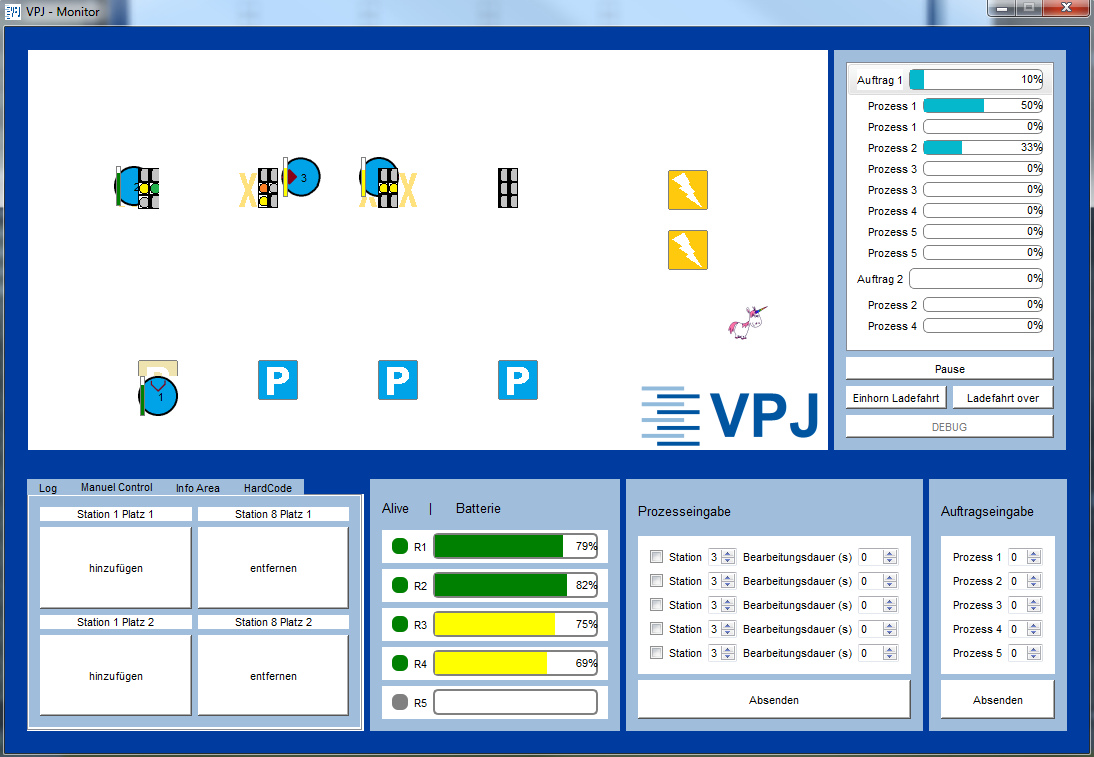
\includegraphics[width=1\textwidth]{Abbildungen/Gesamtprogramm.png}
    \caption{Übersicht Visualisierung}		
    \label{fig:Gesamtprogramm}
\end{figure}

\begin{figure}[htb]
    \centering
    \includegraphics[width=1\textwidth]{Abbildungen/GesamtprogrammROT.png}
    \caption{Übersicht Visualisierung im Hard-Code Modus}		
    \label{fig:GesamtprogrammROT}
\end{figure}

\section{Live-View}

\begin{figure}[htb]
    \centering
    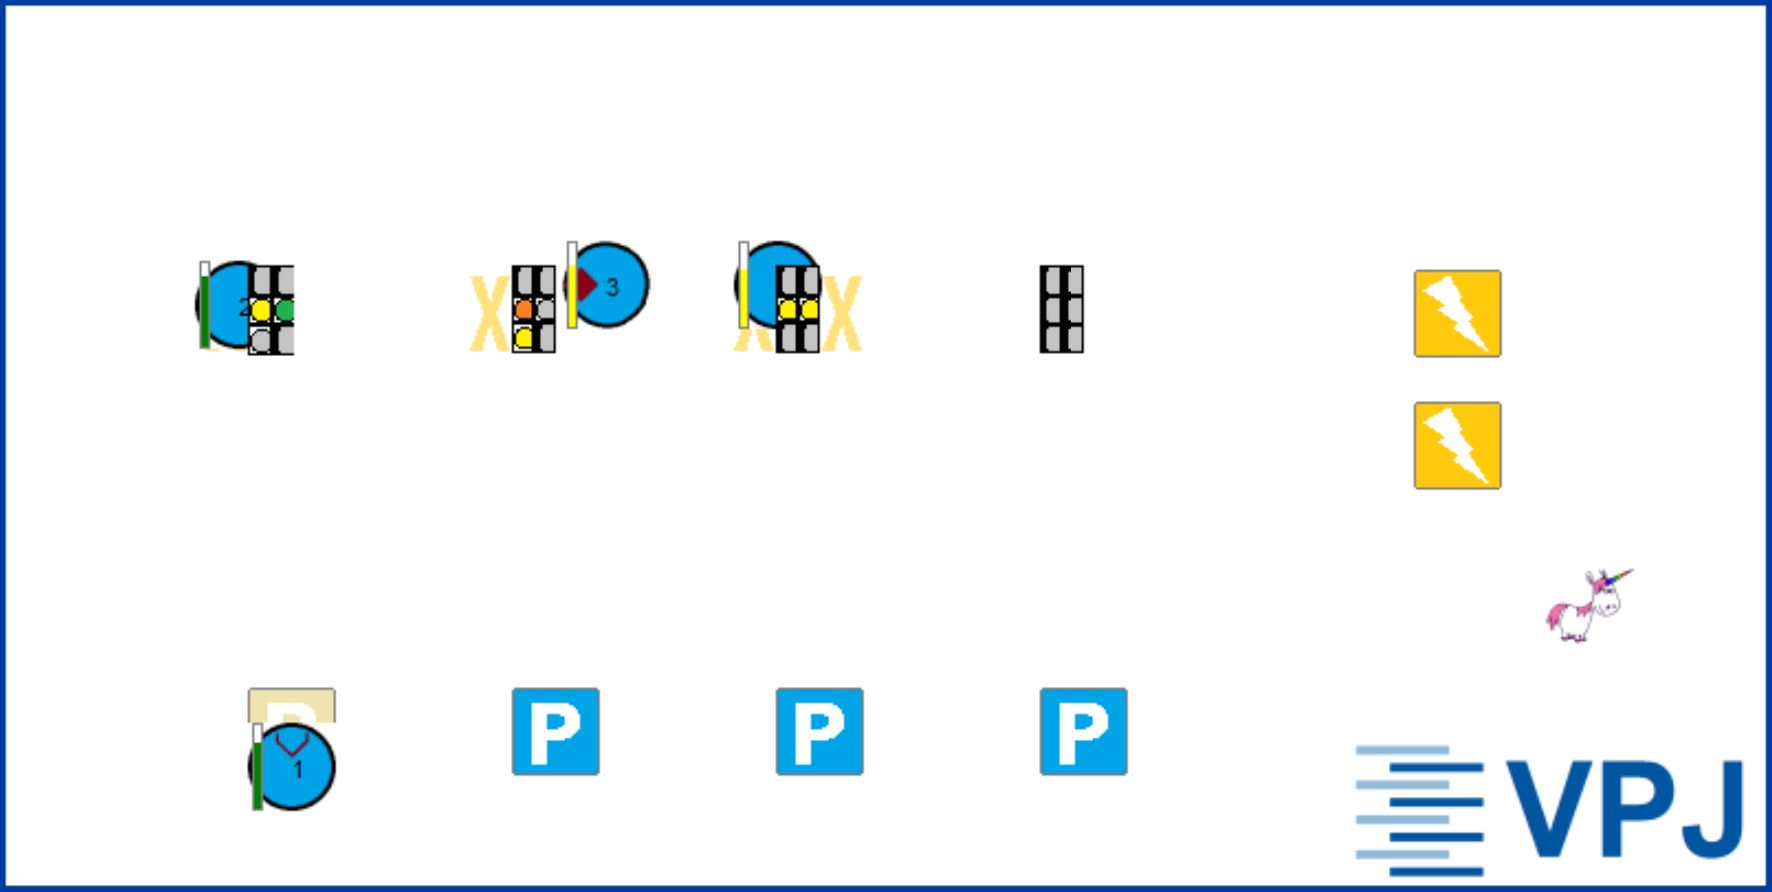
\includegraphics[width=0.9\textwidth]{Abbildungen/LiveView.png}
    \caption{Visualisierung Live-View}		
    \label{fig:LiveView}
\end{figure}

\begin{figure}[htb]
    \centering
    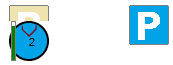
\includegraphics[width=0.4\textwidth]{Abbildungen/Parkplatz.png}
    \caption{Visualisierung Parkplatz}		
    \label{fig:Parkplatz}
\end{figure}

\begin{figure}[htb]
    \centering
    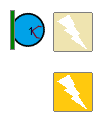
\includegraphics[width=0.25\textwidth]{Abbildungen/Laden.png}
    \caption{Visualisierung Ladestation}		
    \label{fig:Ladestation}
\end{figure}

\begin{figure}[htb]
    \centering
    
\includegraphics[width=0.2\textwidth]{Abbildungen/Station.png}
    \caption{Station mit verschiedenen Arbeitsplatzstati}		
    \label{fig:Station}
\end{figure}

\begin{figure}[htb]
    \centering
    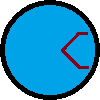
\includegraphics[width=0.1\textwidth]{Abbildungen/RobotinoGoffen.png}
    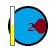
\includegraphics[width=0.1\textwidth]{Abbildungen/RobotinoGZu.png}
    
\includegraphics[width=0.1\textwidth]{Abbildungen/RobotinoDefect.png}
    \caption{Roboter in verschiedenen Stati (vlnr: Greifer offen, Greifer geschlossen, Defekt)}		
    \label{fig:Robotino}
\end{figure}

\section{Auftragsübersicht}
\label{sec:Auftragsuebersicht}

\begin{figure}[htb]
    \centering
    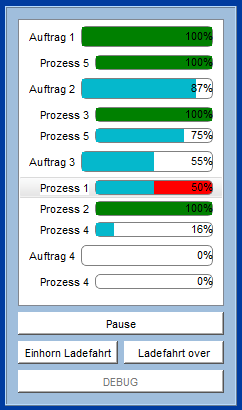
\includegraphics[width=0.4\textwidth]{Abbildungen/Auftragsfortschritt.png}
    \caption{Auftragsfortschritt}		
    \label{fig:Auftragsfortschritt}
\end{figure}

\begin{figure}[htb]
    \centering
    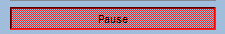
\includegraphics[width=0.4\textwidth]{Abbildungen/Pause.png}
    \caption{Pause Button gedrückt}		
    \label{fig:Pause}
\end{figure}

\section{Tab-View}

\begin{figure}[htb]
    \centering
    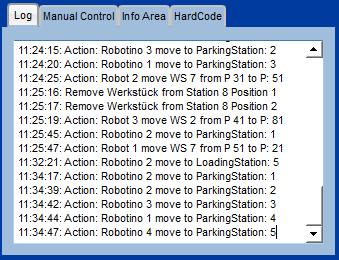
\includegraphics[width=0.6\textwidth]{Abbildungen/Log.png}
    \caption{Tab: Log View}		
    \label{fig:Log}
\end{figure}

\begin{figure}[htb]
    \centering
    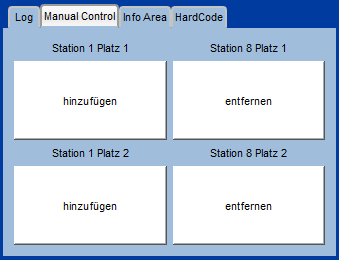
\includegraphics[width=0.6\textwidth]{Abbildungen/ManualControl.png}
    \caption{Tab: Manual Control}		
    \label{fig:ManualControl}
\end{figure}

\begin{figure}[htb]
    \centering
    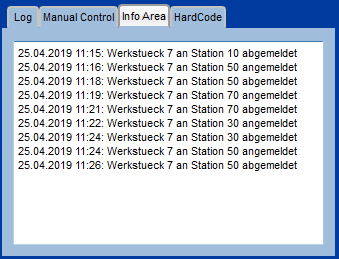
\includegraphics[width=0.4\textwidth]{Abbildungen/TimestampsWerkstueck.png}
    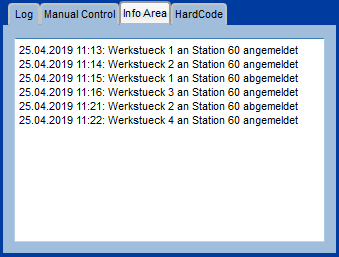
\includegraphics[width=0.4\textwidth]{Abbildungen/TimestampsStation.png}
    \caption{Tab: Info Area}		
    \label{fig:InfoArea}
\end{figure}

\subsection{Hard-Code Bereich}
\label{sec:HardCode}

\begin{figure}[htb]
    \centering
    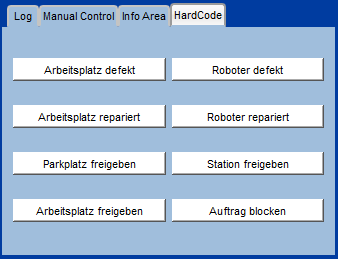
\includegraphics[width=0.6\textwidth]{Abbildungen/HardCode.png}
    \caption{Tab: Hard-Code}		
    \label{fig:HardCode}
\end{figure}

\section{Roboterstatus}

\begin{figure}[htb]
    \centering
    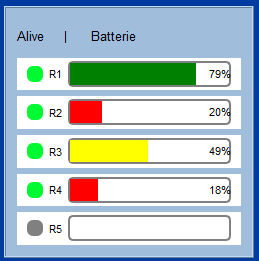
\includegraphics[width=0.5\textwidth]{Abbildungen/Batterie.png}
    \caption{Batterie und Statusanzeige}		
    \label{fig:Batterie}
\end{figure}

\begin{figure}[htb]
    \centering
    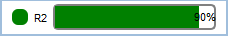
\includegraphics[width=0.4\textwidth]{Abbildungen/BatterieAlive1.png}
    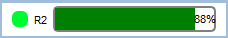
\includegraphics[width=0.4\textwidth]{Abbildungen/BatterieAlive2.png}
    \caption{Roboterstatus-LED blinkend}		
    \label{fig:Led}
\end{figure}

\section{Prozesseingabe}
\label{sec:Prozesseingabe}

\begin{figure}[htb]
    \centering
    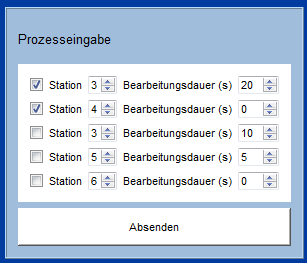
\includegraphics[width=0.5\textwidth]{Abbildungen/Prozesseingabe.png}
    \caption{Visualisierung - Prozesseingabe}		
    \label{fig:Prozesseingabe}
\end{figure}

\section{Auftragseingabe}
\label{sec:Auftragseingabe}

\begin{figure}[htb]
    \centering
    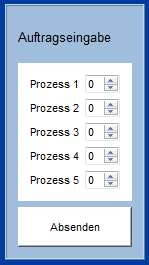
\includegraphics[width=0.25\textwidth]{Abbildungen/Auftragsvergabe.png}
    \caption{Visualisierung - Auftragsvergabe}		
    \label{fig:Auftragsvergabe}
\end{figure}


\section{Benutzerinteraktion}

\subsection{Tooltips}
\label{sec:tooltips}
\inlinetodo {Tooltips mit Bildern her und erlaeeeren}



% !TEX root = ../VPJ.tex

\chapter{Robotersimulation}
\label{sec:Simulation}

Um verschiedene Programmabläufe und Funktionen zu testen, war es wichtig, auch ohne realen Roboter die standardmäßige Programmfunktionalität darstellen zu können. Die Klasse SimulatedRobot erfüllt genau diese Anforderung. 

Mittels einer simulated-Flag kann in der Main-Funktion ein Simulationsbetrieb gestartet werden. In diesem ist kein realer Roboter notwendig, trotzdem findet eine normale Auftragsplanung- und Abarbeitung statt. Die simulated-Flag wird in der Initialisierung dem UDP-Handler übergeben, der die Kommunikation mit den Robotern übernimmt. Somit wird in der Simulation kein Socket erzeugt und verbunden (siehe \ref{sec:UdpHandler}), sondern die Klasse SimulatedRobot genutzt. 

SimulatedRobot enthält eine State-Machine mit 13 Zuständen, die den Roboter ausreichend nachbilden. Weiterhin werden Funktionen für das simulierte Senden des Roboters an den UDPHandler und Timer für die Zustandswechsel bereitgestellt. 

Wie im echten Roboter wird der aktuelle Auftrag und Auftragstyp zwischengespeichert. 

\section{Zustandsdiagramm simulierter Roboter}

Das Zustandsdiagramm in Abbildung \ref{fig:simRobot} beschreibt die Zustände und Transitionen eines simulierten Roboters. Das Diagramm wurde anschließend als State Machine (vgl. \ref{sec:StateMachines}) implementiert. 

\begin{figure}[htb]
    \centering
    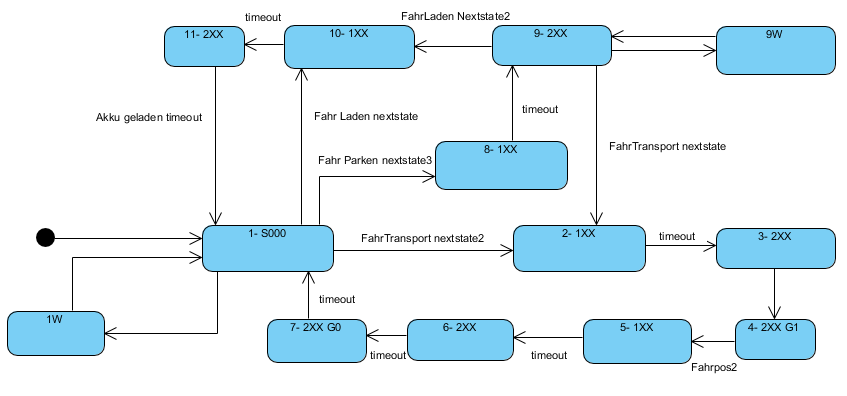
\includegraphics[width=1\textwidth]{Abbildungen/SimulatedRobot.PNG}
    \caption{Ablaufdiagramm des simulierten Roboters}		
    \label{fig:simRobot}
\end{figure}

Da in der Fertigungsplanung für die Vergabe der Aufträge die tatsächliche Position des Roboters nicht berücksichtigt wird, wird im simulierten Roboter ausschließlich die für die Planung benötigte Status- und Greiferinformation nachgepflegt. 

Die Änderung der Statusinformation ist im Diagramm in den Zuständen als Zahl mit zwei folgenden Dont-Care (XX) gekennzeichnet, da die Position keine weitere Relevanz hat. Eine Änderung des Greifers ist mit G0, für Greifer öffnet sich, oder G1 für Greifer schließt sich gekennzeichnet.

Zur Initialisierung wurden ähnlich der State Machine aus Kapitel \ref{sec:StateMachineImplementierung} zunächst alle Zustände und Transitionen hinzugefügt, verknüpft und die State Machine gestartet. 

Der Initialzustand 1 kann über Empfang eines Auftrags zum Laden zu Zustand 10, zum Parken zu Zustand 8 oder zum Transport zu Zustand 2 verlassen werden. Außerdem wird das aktive Abfragen eines Auftrags an den Roboter alle 3 Sekunden über den Zustand 1W getriggert. Über den Wartezustand wird ein bearbeiteter, noch anliegender, Auftrag zurückgesetzt. 

Der Ablauf innerhalb der State-Machine zwischen zwei Aufträgen erfolgt über fest definierte Timer, die Zustandswechsel bewirken und ein Senden des Roboterstatus an den UDP-Handler hervorrufen.

Da innerhalb von Qt keine Events verloren gehen, kann auf ein periodisches Senden, wie der echte Roboter es tut, verzichtet werden.

\subsubsection{Simulierte Ladefahrt}

Wenn in Zustand 1 am simulierten Roboter ein Ladefahrtauftrag anliegt, also ein Auftrag mit der ID 3, so wird direkt in Zustand 10 gewechselt. Es wird an den UDP-Handler ein Status 100 zurückgegeben (auf dem Weg zur Ladestation) und ein Timer von 3 Sekunden gestartet. Nach Ablauf des Timers wird in Zustand 11 der Status 2XX zurückgegeben, was bedeutet, dass die Ladestation erreicht wurde. Nach Ablauf weiterer 5 Sekunden gilt das Laden als beendet und der Roboter geht in Zustand 1 über und sendet Status 000.

\subsubsection{Simulierter Parkvorgang}

Bei einem Parkauftrag in Zustand 1, also ein Auftrag mit der ID 2, wird in Zustand 8 gewechselt. An den UDP-Handler wird, da der simulierte Roboter jetzt auf dem Weg zum Parken ist, als Status 100 zurückgegeben. Nach einer Fahrzeit von 3 Sekunden hat der Roboter sein Ziel erreicht und gibt in Zustand 9 als Status 200 an den UDP-Handler. 

Zustand 9 kann entweder über einen Auftrag mit der ID 3 in Zustand 10 verlassen werden, und eine Ladefahrt wird simuliert, oder mit einem Auftrag der ID 1 in Zustand 2 (Transportauftrag) verlassen werden. 

Über den Wartezustand 9W kann auf weitere Aufträge reagiert werden. Dieser wird alle 3 Sekunden aufgerufen. 

\subsubsection{Simulierter Transport}

Sobald ein simulierter Roboter in Zustand 2 kommt, wird an den UDP-Handler der Status 100 übermittelt, da der Roboter sich auf dem Weg zur ersten Auftragsposition befindet. Nach 3 Sekunden wird in Zustand 3 der Status 2XX gesendet, da der Roboter an der ersten Position angekommen ist. Eine weitere Sekunde später wird das Werkstück gegriffen, was durch senden des Greiferstatus 1 in Zustand 4 übermittelt wird. In Zustand 5 wird über Ablauf eines zweisekündigen Timers der Status 100 gesendet, da sich der Roboter auf dem Weg zur zweiten Station des Auftrags befindet. 

In Zustand 6, der nach 3 Sekunden bearbeitet wird, wird zunächst der Status auf 2XX gesetzt, da der Roboter angekommen ist. Nach einer Sekunde wird über Zustand 7 der Greifer geöffnet und der Greiferstatus auf 0 zurückgesetzt. Zwei Sekunden später wird wieder in Zustand 1 auf einen neuen Auftrag gewartet. 

\chapter{Datenbank}\label{kap:Datenbank}
\section{Aufgabe der Datenbank}\label{kap:ZielDerDatenbank}
Die Datenbank soll den aktuellen Zustand der Produktionsanlage abbilden. Dazu gehören die Betriebsmittel, wie zum Beispiel die Fertigungs-Stationen oder die Roboter mit ihren aktuellen Status und der jeweiligen Ladung der Akkumulatoren. Es sollen auch die Verwaltungsdaten, wie Aufträge und Produktionsprozesse in der Datenbank gespeichert werden. Neben dem aktuellen Zustand der Produktionsanlage sollen auch die Fertigungsabläufe dort gespeichert werden. Dies beinhaltet in erster Linie eine Verfolgung der Werkstück durch Timestamps für das An- und Abmelden der Werkstück an den Bearbeitungs-Stationen. Es wird ebenso der Fortschritt, den ein Werkstück im Fertigungsprozess und ein Auftrag insgesamt gemacht hat, gespeichert. Eine weitere Aufgabe der Datenbank ist der Austausch von Daten zwischen dem Fertigungsrechner und der Fertigungsplanung. Alle Daten die zwischen diesen beiden Rechnern ausgetauscht werden, werden in die Datenbank geschrieben.
 
\section{Konzept} \label{kap:DatenbankKonzept}
Aus der realen Fertigungsanlage wird ein konzeptionelles Modell als Entität-Relation\-ship\--Diagramm modelliert. Das so modelliert ER-Diagramm ist in Abbildung \ref{fig:ER-Diagramm} zu sehen. Dazu werden insbesondere die Aufgaben aus Abschnitt \ref{kap:ZielDerDatenbank} berücksichtigt. Zur Qualitätssicherung wird sich an den drei gängigen Normalisierungsformen für Datenbanken orientiert. Anschließend wird das konzeptionelle Modell in ein logisches Datenschema überführt. Das Datenschema soll den Ansprüchen eines relationalen Datenbankmodells entsprechen. Zur Erstellung des Datenschemas wird die MySQL-Workbenche genutzt und deren Möglichkeit ein relationales Datenbankmodell grafisch zu entwerfen.
\begin{figure}[h]
	    \centering
	    \includegraphics[width=0.8\linewidth]{Bilder/ERChanDiagramm.png}
        \caption{Entität-Relationship-Diagramm}
        \label{fig:ER-Diagramm}
\end{figure}
 \section{Konzeptionelles Modell}
Zur Erstellung des konzeptionellen Modells wird für jede Betriebsmittelklasse der realen Anlage ein Entitätstyp angelegt. Es werden folgende Entitätstypen zur Repräsentation von Betriebsmitteln angelegt: Roboter, Arbeitsplatz, Parkplatz und Werkstück. Die vier Entitätstypen enthalten die zu speichernden Attribute der Betriebsmittel. So sollen für das Betriebsmittel Roboter zum Beispiel die Attribute \glqq Akkuleistung\grqq{}  und \glqq Status\grqq{}  gespeichert werden. Neben den Entitätstypen für die realen Betriebsmittel werden auch Entitätstypen für die Verwaltungsdaten, die zur Fertigungsplanung benötigt werden, angelegt. Hierzu zählen die Entitätstypen: Auftrag und Produktionsprozess. Der Entitätstyp Timestamp dient zur Speicherung der Fertigungsabläufe. Der Entitätstyp taggen dient ausschließlich zur Kommunikation zwischen der Fertigungsplanung und dem Programm für die Ansteuerung der RFID-Schreib-Lese-Köpfe. 

Zur Identifizierung der einzelnen Entitäten enthält jeder Entitätstyp mindestens ein Attribut oder eine Kombination von Attributen, die die Entitäten eindeutig unterscheiden. Viele der hier beschriebenen Entitätstypen haben ein aus der realen Welt abgeleitetes Attribut, wodurch die Entitäten unterschieden werden. So ist zum Beispiel die Roboter ID ein Wert der sich aus der Nummerierung der Roboter in der realen Welt ableitet. Es gibt allerdings auch Entitätstypen die eigentlich kein einzelnes Attribut haben, dass sie eindeutig unterscheidet. Als Beispiel hierfür kann der Timestamp genannt werden, wo sowohl der Zeitstempel als auch der Status einen Entität nicht eindeutig identifizieren. Erst in Kombination mit der Beziehung zu einem Werkstück kann der Zeitstempel die Entitäten eindeutig unterscheiden. Zur einfacheren Handhabung des Timestamps wird dem Entitätstyp ein zusätzliches Attribut \glqq id\_Timestamp\grqq{}  hinzugefügt. Dabei handelt es sich um eine laufende Nummer die keinen zusätzlichen Informationen speichert sondern nur der einfacheren Verwaltung dient. Die Attribute oder Kombinationen von Attributen die die Entitäten eines Entitätstyps eindeutig unterscheiden werden Schlüssel genannt. Wie schon beim Timestamp beschrieben, wurde darauf geachtet das jeder Entitätstype nur ein Attribut als Schlüssel hat.
 
Da die Betriebsmittel der realen Welt, ebenso wie die Daten der Fertigungsplanung oder die Fertigungsabläufe, in Beziehung zu einander stehen, werden die Entitätstypen mit Beziehungstypen verbunden und so die jeweilige Beziehung deutlich gemacht. Es gibt je nach Art der Beziehung verschiedene Beziehungstypen. Es werden Beziehungstyp-Richtungen mit Kardinalität 1 oder Kardinalität N verwendet. Wobei die Beziehungstyp-Richtungen mit der Kardinalität 1 sowohl optional als auch nicht-optional vorkommen. Alle vorkommenden Beziehungstypen sind in Tabelle \ref{tab:Beziehungstypen} aufgeführt. Die dort aufgeführten Beziehungen gelten natürlich umgekehrt genauso. Hat Auftrag zu Werkstueck eine 1:CN Beziehung, so hat Werkstueck zu Auftrag eine CN:1 Beziehung. Für die Beziehung zwischen einem Timestamp und einem Werkstueck bedeutet das zum Beispiel, dass ein Timestamp immer zu genau einem Werkstueck gehört, das Werkstueck aber keinen, einen oder mehrere Timestamps haben kann. Es sich also um einen 1:CN Beziehungstyp handelt. Ein Parkplatz hingegen kann immer nur für einen oder keinen Roboter reserviert sein. Genauso kann ein Roboter immer nur an einem oder an keinem Parkplatz sein. Es handelt sich also um eine C:C Beziehung. 

\begin{table}[htbp]
    \centering	
    \captionof{table}{Beziehungstypen}
    \begin{tabular}{|p{4cm}|p{8cm}|} 
    \hline Beziehungstyp &  zwischen  \cr 
    \hline \hline  C:C &  taggen zu werkstueck\newline roboter zu parkplatz \newline roboter zu werkstueck \cr
    \hline C1:CN  & arbeitsplatz zu roboter \newline arbeitsplatz zu werkstueck \cr
    \hline 1:CN  & werkstueck zu timestamp \newline arbeitsplatz zu timestamp \newline auftrag zu werkstueck \newline produktionsprozess zu werkstueck \cr
    \hline 
    \end{tabular}
    \newline
    \label{tab:Beziehungstypen}
\end{table}

Beim entwerfen des Datenmodells mit einem Entity-Relationship-Diagramm, gilt es verschiedene Punkte zu beachten. Besonders wichtig ist es, Redundanz bei Attributen zu vermeiden. Bei Redundanz treten verschiedene Probleme auf. So müssen die selben Daten mehrfach in die Datenbank geschrieben werden und es wird außerdem unnötig Speicherplatz belegt. Diese Probleme sind aufgrund der kleinen Datenmenge und der geringen Anzahl an Usern bei der hier beschriebenen Produktionsanlage wenig relevant. Redundanz ist auch deshalb zu vermeiden, weil sich ein Problem ergibt, wenn inkonsistente Daten entstehen, weil nicht an allen Stellen, die mehrfach vorhandenen Daten geändert wurden. Um Redundanzen in der Datenbank zu vermeiden, wird das Datenbankmodell normalisiert. Das Normalisieren ist im Abschnitt \ref{kap:Normalisierung} beschrieben.
Ebenso ist darauf zu achten keine, redundanten Beziehungstypen zu modellieren. Eine Redundanz kann immer dann vermutetet werden, wenn zwei Wege von einem Entitätstyp zu einem anderen Entitätstyp möglich sind. Beispielhaft sei hier der Entitätstyp Timestamp genannt, der sowohl eine direkte Beziehung zum Entitätstyp Werkstueck als auch eine indirekte Beziehung über den Entitätstyp Arbeitsplatz hat. Da es sich bei den beiden Beziehungen des Timestamps allerdings um zeitlich abgeschlossene Vorgänge handelt und die Beziehung zwischen Arbeitsplatz und Werkstück den aktuellen Zustand speichert, kann von der Beziehung des Timestamps zum Arbeitsplatz nicht auf das dazugehörige Werkstück geschlossen werden, so dass die direkte Beziehung zum Werkstück notwendig ist.\cite{Jarosch:2016}



\subsection{Normalisierung }\label{kap:Normalisierung}
Anhand von Normalisierungsstufen kann die Qualität eines Datenmodells beurteilt werden. Zur Qualitätssicherung wurden die ersten 3 Normalisierungsstufen auf das in Abschnitt \ref{kap:DatenbankKonzept} beschriebene und in Abbildung \ref{fig:ER-Diagramm} dargestellte konzeptionelle Datenmodell angewandt. Durch die Anwendung der 3 Normalisierungsstufen entsteht ein Datenmodell, dass in der 3. Normalform vorliegt. Das Vorliegen in der 3. Normalform bietet auch bei der Überführung in das relationale Datenbank-Modell Vorteile Beziehungsweise ist bei Stufe 1 sogar Voraussetzung.

\subsubsection*{1. Normalform}
Die erste Normalform besagt das eine Entität keine Attribute besitzen darf die zur gleichen Zeit mehrere Werte annehmen können. So würde es zum Beispiel gegen die 1. Normalform verstoßen wenn die Zeitstempel als Attribut des Werkstücks angelegt worden wären, da dieses Attribut, je nach dem wie viele Stationen das Werkstück schon durchlaufen hat, mehrere Werte annehmen könnte. Um die 1. Normalform zu erreichen, werden Attribute die mehrere Werte annehmen können aus dem Entitätstyp herausgelöst und bilden einen eigenen Entitätstyp, der durch einen Beziehungstyp mit dem ursprünglichen Entitätstyp verbunden ist. Dabei hat die Beziehungstyp-Richtung "`Ursprüngliche Entitätstyp zu neuem Entitätstyp"' die Kardinalität N oder CN.
Angewandt auf das Beispiel des Zeitstempels wurde, wie in Abbildung \ref{fig:ER-Diagramm} zu sehen ist, der Zeitstempel in den neuen Entitätstype Timestamp ausgelagert. Der Beziehungstyp-Richtung von Werkstück zu Timestamp ist CN.
Ein Wert welcher nicht aus einer Liste besteht oder auf andere Weise aus mehreren Werten zusammengesetzt ist wir als atomarer Wert bezeichnet. Für ein relationales Datenbank-Modell gilt: Jeder Wert eines Attributes muss ein atomarer Wert sein.\cite{Jarosch:2016}

\subsubsection*{2. Normalform}
Damit ein Datenmodell in der 2. Normalform vorliegt, muss es sich in der ersten Normalform befinden. Zusätzlich darf jedes Attribut ausschließlich vom Gesamtschlüssel eines Entitätstyps funktional Abhängig sein. Funktionale Abhängigkeit bedeutet, dass aus dem Wert von Attribut A sich automatisch der Wert von Attribut B ergibt. Zum Verdeutlichen der zweiten Normalform nutze ich ein etwas konstruiertes Beispiel: Angenommen die Produktionsanlage fährt mit zwei verschiedenen Typen von Robotern. Mit jeweils zwei alten Festo-Robotern und zwei neuen von Studenten entwickelten Robotern. Die ID der Roboter setzt sich nun aus zwei Ziffern zusammen die jeweils ein eigenes Attribut bilden und zusammen den Gesamtschlüssel für den Entitätstyp Roboter. Die erste Ziffer wäre dabei entweder eine 1 für die Festo-Roboter oder eine zwei für die neuen Roboter. Die zweite Ziffer ist eine laufende Nummer. Wird jetzt zusätzlich das Baujahr gespeichert und sind die Roboter eines Typs jeweils im gleichen Jahr gebaut so liegt eine funktionale Abhängigkeit zwischen dem Attribut Baujahr und dem Teilschlüssel erste Ziffer vor. Um die zweite Normalform nun herzustellen wird der Teilschlüssel und das abhängige Attribut herausgelöst und sie bilden einen neuen Entitätstyp. Die zweite Normalform verringert Redundanzen innerhalb des Datenmodells.\cite{Heuer:2001}

\subsubsection*{3. Normalform}
Damit ein Datenmodell in der 3. Normalform vorliegt muss es sich in der 2. Normalform befinden und zusätzlich darf eine Attribut eines Entitätstyps nicht transitiv funktional abhängig sein.  So wäre es zum Beispiel möglich, die Attribute des Entitätstyps Produktionsprozesses mit im Entitätstyps Werkstück zu speichern. Es läge dann allerdings eine transitive funktionale Abhängigkeit zwischen den Werten der Attribute Station 1 bis 5 und Dauer Station 1 bis 5 und dem Schlüssel RFID Werkstück vor, da die Attribute Station 1 bis 5 und Dauer Station 1 bis 5 funktional von der id\_Produktionsprozess abhängig wären. Die id\_Produktionsprozess wiederum wäre funktional abhängig vom Schlüssel RFID Werkstück. Deshalb wird dieser Teil herausgelöst und bildet einen eigenen Entitätstyp. Die dritte Normalform verringert die Gefahr von Redundanzen im Datenmodell.\cite{Heuer:2001}

\section{Relationales Datenbankmodell}\label{kap:relationales_Datenbankmodell}
Bei einer MySQL-Datenbank handelt es sich um eine relationale Datenbank. Dabei entspricht eine Entität aus dem ER-Diagramm einem Tupel von Werten und der Entitätstyp einem Relationstyp. 

So lässt sich nun die Mengen aller Entitäten eines Entitätstyps als Tabelle darstellen. Dabei entsprechen die Überschriften der einzelnen Spalten den Namen der Attribute. Was im ER-Diagramm Attribute genannt wurde, wird nun Eigenschaften genannt. Eine Zeile repräsentiert dann jeweils eine Entität Beziehungsweise ein Tupel von Werten. Wie schon beim ER-Diagramm hat jeder Relationstyp ein oder mehrere Attribute zur eindeutigen Identifizierung der jeweiligen Tupel, die im relationalen Datenbankmodell als Primärschlüssel bezeichnet werden und dem Schlüssel im ER-Diagramm entsprechen. Beziehungstypen werden über sogenannte Fremdschlüssel realisiert. Fremdschlüssel stellen eine zusätzliche Spalte in einer Tabelle da. Ist in einer Tabelle ein Fremdschlüssel eingetragen, referenziert dieser auf eine  Zeile einer anderen Tabelle und stellt so die Beziehung her. Dabei muss stets die referenzielle Integrität dieser Verweise gewährleistet sein, dass bedeutet das ein Fremdschlüssel immer auf eine vorhandene Zeile einer anderen Tabelle referenzieren muss oder mit einem NULL-Marker belegt sein muss. 

\section{Zugriff auf die Datenbank}\label{kap:DatenbankZugriff}
Die MySQL-Datenbank ist auf einem Server, der auf dem Fertigungsrechner läuft, implementiert. Es gibt zwei User die Zugriff auf die Datenbank benötigen. Das ist zum einen die Fertigungsüberwachung, die das Auslesen der RFID-Tags übernimmt und die Fertigungsplanung. Die Fertigungsüberwachung befindet sich auf dem selben Rechner wie der Server der Datenbank. Die Fertigungsplanung ist auf einem anderen Rechner realisiert und über Ethernet mit dem Fertigungsrechner verbunden. Die Fertigungsplanung ist mit Qt ausgeführt und hat über eine eingebundene Bibliothek über Ethernet direkten Zugriff auf die Datenbank. 

Die Fertigungsüberwachung läuft auf einer Soft-SPS auf dem Fertigungsrechner und ist mit CODESYS programmiert. Ein direkter Zugriff von der Soft-SPS auf die Datenbank ist nicht möglich. Ein Zugriff könnte über einen OPC-Server erfolgen. OPC (Open Platform Communications) ist eine standardisierte Softwareschnittstelle. Sie ermöglicht den Datenaustausch zwischen Steuerungen verschiedener Hersteller aus der Automatisierungstechnik. Hier wurde allerdings ein anderes Verfahren, speziell für den Zugriff auf Datenbanken von Steuerungen aus der Automatisierungstechnik, angewandt. Es handelt sich dabei um den SQL4Automation Connector der Firma Inasoft Systems GmbH. Dieser wurde speziell für den Zugriff von Speicherprogrammierbaren Steuerungen auf eine Datenbank entwickelt und ermöglicht sowohl Lese- als auch Schreibbefehle in SQL direkt auf der SPS zu programmieren. Für die verwendete Steuerung ist schon eine fertige Bibliothek vorhanden, was die Anwendung deutlich erleichtert. In Abbildung \ref{fig:DatenbankZugriffUebersicht} ist schematisch dargestellt, wie auf die Datenbank zugegriffen wird.

\begin{figure}[ht]
	    \centering
	    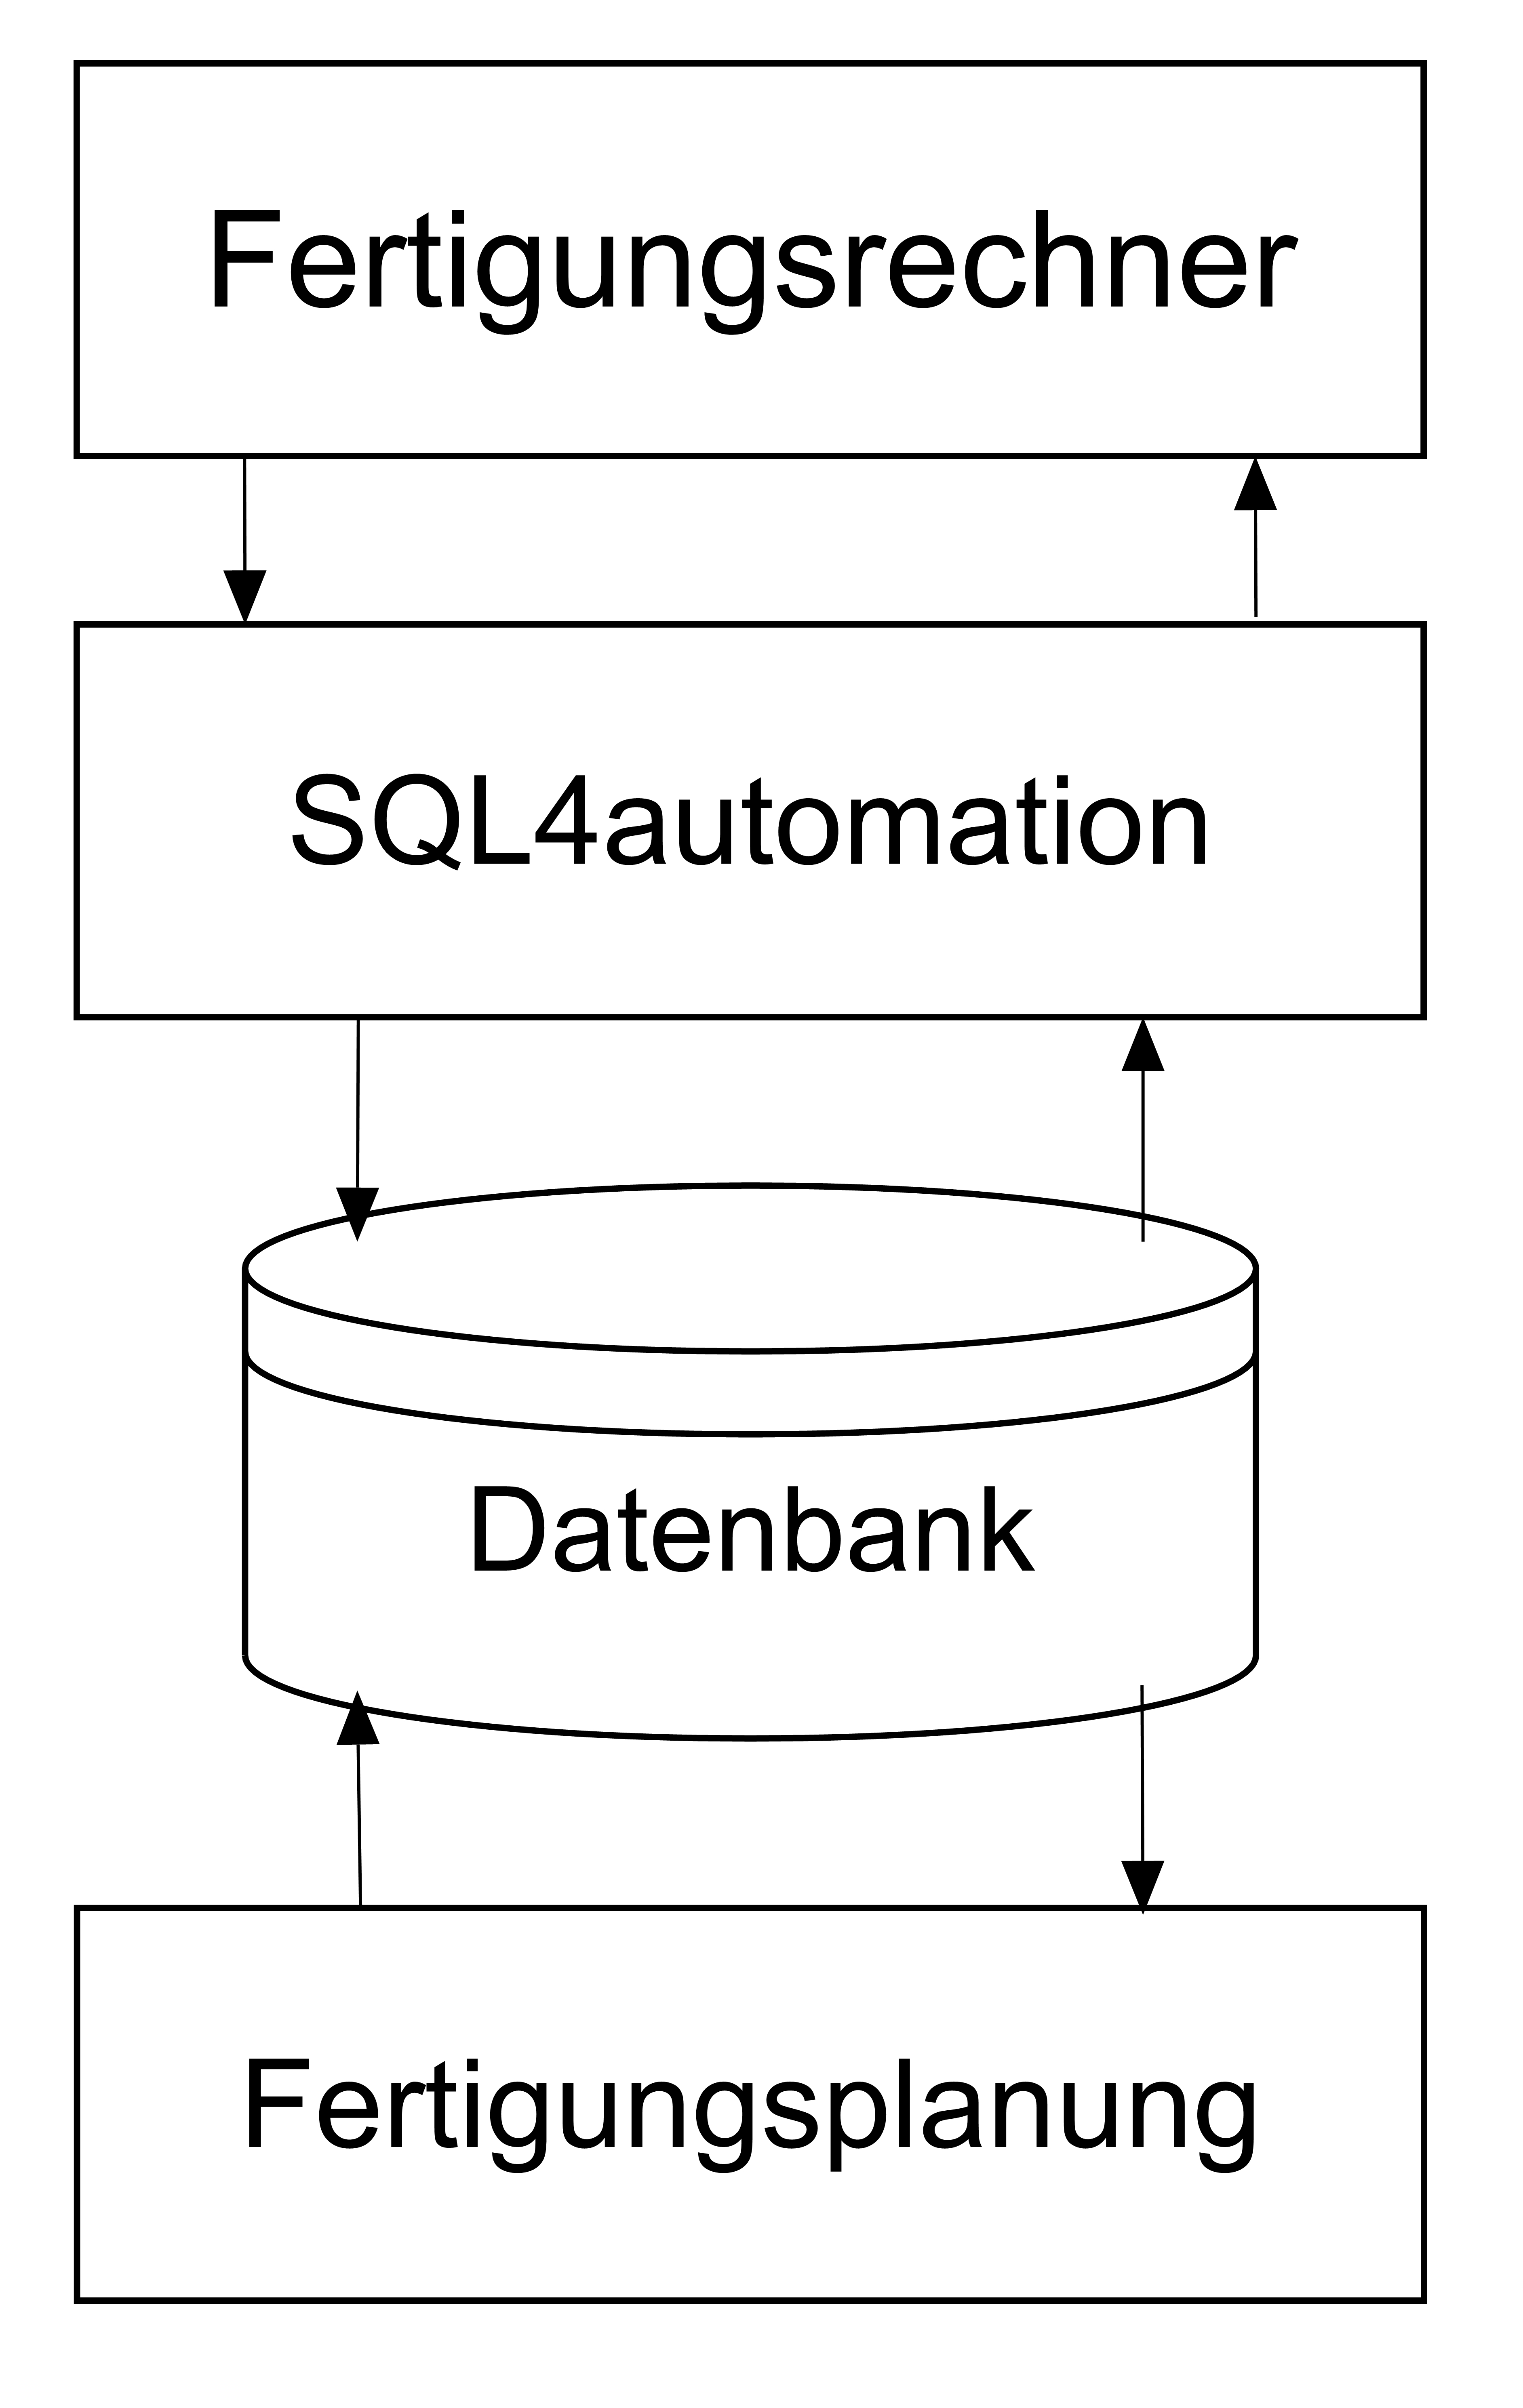
\includegraphics[width=0.4\linewidth]{Bilder/Datenbankdiagramm.png}
        \caption{Schematische Darstellung des Datenbankzugriffs}
        \label{fig:DatenbankZugriffUebersicht}
\end{figure}


\section{Umsetzung des entwickelten Modells}
Zunächst wurde anhand des in Abschnitt \ref{kap:DatenbankKonzept} beschriebenen Konzeptes das ER-\-Dia\-gramm der Datenbank grafisch entwickelt. Das so entstandene ER-Diagramm, ist in Abbildung \ref{fig:ER-Diagramm} zu sehen. Die Entwicklung des ER-Diagramms erfolgte in enger Absprache mit der Fertigungsplanung, da diese einer von zwei Nutzern der Datenbank ist.
 
\begin{figure}[ht]
	    \centering
	    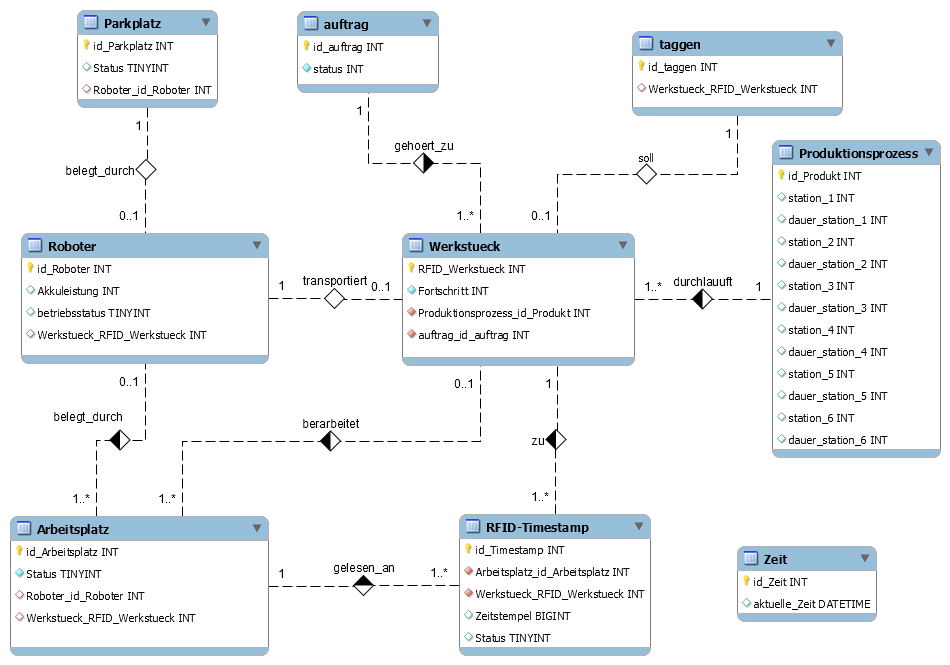
\includegraphics[width=1\linewidth]{Bilder/DB_Modell.png}
        \caption{Grafisches Modell der Datenbank}
        \label{fig:ER-Diagramm_Worbenche}
\end{figure}
 
Zum Erstellen der Datenbank wurde das Tool MySQL-Workbenche vom Entwickler Oracle Corporation genutzt. Dieses Tool ermöglicht die visuelle Entwicklung, Erstellung und Bearbeitung einer Datenbank. Es können außerdem MySQL-Befehle, zum Beispiel zum Testen, ausgeführt werden. Die visuelle Entwicklung erfolgt über die grafische Eingabe des aus dem ER-Diagramm entwickelten relationalen Datenbankmodells wie in Abbildung \ref{fig:ER-Diagramm_Worbenche} dargestellt. In der Tabelle \ref{tab:ER-Erklaerung} sind die Symbole, die durch die MySQL-Workbenche verwendet werden, beschrieben.
%\begin{comment}
\begin{table}[ht]%{1\textwidth}
    \centering	
			\renewcommand{\arraystretch}{2}

    \captionof{table}{Zeichenelegende MySQL-Workbench Modell}
    \begin{tabular}{|p{1.8cm}|p{8cm}|} 

    \hline Zeichen &  Bedeutung  \cr 
    \hline \hline   
\includegraphics[width=0.5cm,]{Bilder/ER/Primaerschluessel.PNG} &  Primärschlüssel \cr
    \hline 
\includegraphics[width=0.5cm,]{Bilder/ER/EigenschaftNN.PNG}  & Eigenschaft (darf nicht NULL sein) \cr
    \hline 
\includegraphics[width=0.5cm,]{Bilder/ER/Eigenschaft.PNG}  & Eigenschaft \cr
    \hline 
\includegraphics[width=0.5cm,]{Bilder/ER/FremdschluesselNN.PNG}  &  Fremdschlüssel (darf nicht NULL sein)\cr
    \hline 
\includegraphics[width=0.5cm,]{Bilder/ER/Fremdschluessel.PNG}  & Fremdschlüssel \cr
    \hline 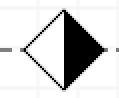
\includegraphics[width=0.5cm,]{Bilder/ER/1zuN.PNG}  & 1:N Beziehung \cr 
    \hline 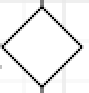
\includegraphics[width=0.5cm,]{Bilder/ER/1zu1.PNG} &  1:1 Beziehung \cr
    \hline 
    \end{tabular}
    \newline
    \label{tab:ER-Erklaerung}
\end{table}
%\end{comment}
Es können dort die Entitätstypen, welche in das relationale Datenbankmodell transformiert einer Tabelle entsprechen, angelegt werden. Jeder Tabelle können ein Primärschlüssel und Eigenschaften zugewiesen werden. Sowohl dem Primärschlüssel, als auch den Eigenschaften muss ein Datentyp zugewiesen werden. Es können auch weitere Festlegungen für die Eigenschaften getroffen werden. So kann eine Eigenschaft als \glqq NOT NULL\grqq{}  festgelegt werden, was bedeutet, dass beim Anlegen einer neuen Entität beziehungsweise einer neuen Zeile in der Tabelle diese Eigenschaft immer gesetzt werden muss und auch nicht später gelöscht werden kann. So muss zum Beispiel ein Parkplatz immer einen Status haben. Beim Produktionsprozess, der nicht immer die selbe Länge hat, ist es nicht notwendig das alle Eigenschaften immer einen Wert haben. So brauch ein Produktionsprozess mit nur 4 Stationen die Eigenschaften \glqq station\_5\grqq{}  und \glqq dauer\_station\_5\grqq{}  nicht. Der Primärschlüssel muss selbstverständlich immer vergeben werden und darf nicht mit einem  NULL-Marker belegt sein.
Auch Beziehungstypen können in der MySQL-Workbenche abgebildet werden. Wird ein Beziehungstyp angelegt, so erzeugt dieser automatisch den, wie in Abschnitt \ref{kap:relationales_Datenbankmodell} beschrieben, dazugehörigen Fremdschlüssel in den jeweiligen Tabellen. Je nach Beziehungstyp dürfen diese durch einen NULL-Marker belegt  sein oder müssen eine Wert haben. So kann bei einer optionalen C1:CN Beziehung, wie sie zum Beispiel von Arbeitsplatz zu Roboter besteht, das Feld für den Fremdschlüssel auch \glqq NULL\grqq{}  sein. Bei einer 1:CN Beziehung, wie vom Auftrag zum Werkstueck, darf der Fremdschlüssel \glqq auftrag\_id\_auftrag\grqq{}  beim Werkstück nicht mit einem NULL-Marker belegt sein, da jedes Werkstück einem Auftrag zugeordnet werden muss.
 
Nach dem grafischen Entwurf der Datenbank kann mittels der Option \glqq Forward Engineer to Database\grqq{}  aus dem grafischen Modell automatisch der entsprechende Code für die Datenbank erstellt werden und die Datenbank ohne weitere Programmierung implementiert werden. Auch nachträgliche Änderungen oder Erweiterungen an der Datenbank können direkt im grafischen Modell erfolgen und über die \glqq Forward Engineer to Database\grqq{}  Option direkt eingepflegt werden. So bleibt das grafische Modell und die Datenbank immer auf dem selben Stand. Es ist keine zusätzliche Pflege der Dokumentation während des Entwicklungsprozess nötig. 
 
Nach dem Erstellen der Datenbank lässt sich die Struktur der Datenbank im Navigator der MySQL-Workbenche betrachten. Zum Befüllen der Datenbank lassen sich über das Abfragefenster MySQL-Befehle, wie zum Beispiel \glqq INSERT INTO\grqq{},  ausführen. Beim Befüllen ist insbesondere darauf zu achten, die Tabellen in der richtigen Reihenfolge zu befüllen. So kann ein Werkstück zum Beispiel erst angelegt werden, wenn der dazugehörige Auftrag bereits erstellt wurde.
 
Über das Abfragefenster lassen sich auch die MySQL-Befehle, die später im CODE\-SYS-Programm auf der Soft-SPS sowie im mit Qt entwickelten Programm auf dem Fertigungsrechner implementiert werden, testen. Auf die MySQL-Befehle die für Qt entwickelt wurden wird in \ref{kap:MySQLBefehle} eingegangen. 

Das Erstellen der MySQL-Befehle lief nach und nach parallel zur Entwicklung der beiden User-Programme der Datenbank. Zunächst wurde die Anforderung an den Befehl festgelegt. Anschließend wurde der Befehl erstellt und mit der MySQL-Workbenche getestet. Nach dem erfogreichen Test wurde der Befehl in seine Zielumgebung, also CODESYS oder Qt, portiert und dort erneut getestet. Beim Testen der Befehle ist insbesondere der Error-Code interessant. Er liefert wichtige Hinweise warum ein Befehl nicht funktioniert. Der Error-Code kann anhand von Error-Code Listen dekodiert werden. Für die Tests in der MySQL-Workbenche übernimmt das dekodieren die Entwicklungsumgebung.

\section{MySQL-Befehle für die Fertigungsplanung}\label{kap:MySQLBefehle}
Im folgenden Abschnitt wird zunächst allgemein beschrieben wie die in Qt verwendeten MySQL-Befehle aufgebaut sind und anschließend jeweils ein Befehl der drei Klassen Getter, Setter und Update näher beschrieben. Hier wird nur auf den Aufbau der MySQL-Befehle eingegangen. Wie der Aufruf der Funktion aus Qt heraus funktioniert ist in Abschnitt \ref{sec:Databasehandler} beschrieben.

Es hat sich für die Implementierung in Qt herausgestellt, dass es sinnvoll ist zunächst mit einem SET-Befehl eine Variable zu deklarieren und ihr einen Wert zuzuweisen. Das erhöht die Lesbarkeit des Codes, da die eigentliche Abfrage nicht zerschnitten werden muss. 
\subsection{Getter}\label{kap:MySQLGetter}
Im Folgenden wird beispielhaft ein MySQL-Befehl aus einem Getter in Qt beschrieben: Ein Getter fragt Werte aus der Datenbank ab, ohne diese zu verändern.
Im Listing \ref{lst:MySQLQtGetter} ist der Code für die Abfrage, ob und welcher Arbeitsplatz an einer Station frei ist, dargestellt. Der Befehl befindet sich in der Funktion GetZielStationsplatzFree(int Station). Die Zuweisung zur Variable \glqq @Station1\grqq{} entspricht dabei dem der Funktion übergebenen Wert mit 10 multipliziert, da die einzelnen Plätze wie in Abbildung \ref{fig:Positionskodierung} dargestellt kodiert sind. Diese Abfrage liefert eine 1 zurück wenn beide (Zeile 4) oder der erste (Zeile 5) Arbeitsplatz der entsprechenden Station frei sein. Ist nur der zweite Arbeitsplatz frei liefert die Abfrage eine 2 (Zeile 6) und sollten alle Arbeitsplätze belegt sein, wird eine 0 zurückgeliefert (Zeile 7).
 
\lstset{ 
    keywordstyle        =\bfseries\ttfamily\color{blue},
    basicstyle          =\scriptsize\ttfamily, 
    emphstyle           =\color{red},
    %identifierstyle     =\color{magenta},
    numbers             =left,
    xleftmargin         =15pt,
    backgroundcolor     =\color{newgray},
    showstringspaces    =false,
    language            =SQL
    }	 

\begin{lstlisting}[caption={MySQL-Befehl: Freier Arbeitsplatz }
       \label{lst:MySQLQtGetter}, float=hbt,
       captionpos=t] 
SET @Station1 = station*10; 
SELECT
    (CASE
        WHEN(SUM(id_Arbeitsplatz))=@Station1+1+@Station1+2 THEN 1 
        WHEN(SUM(id_Arbeitsplatz))=@Station1+1 THEN 1 
        WHEN(SUM(id_Arbeitsplatz))=@Station1+2 THEN 2 
        ELSE 0 
    END) 
FROM 
    vpj.arbeitsplatz 
WHERE (id_Arbeitsplatz IN (@Station1+1,@Station1+2) 
        AND Werkstueck_RFID_Werkstueck is NULL);
\end{lstlisting}

Bei den MySQL-Gettern handelt es sich meistens um Abfragen die nur einen Wert zurück liefern und keine ganzen Tabellen, so dass die Rückgabewerte direkt eine Aussage treffen und nicht die  Tabellen erneut durchsucht werden müssen. Ziel war es, die Abfragen so präzise wie möglich zu gestalten, um die Nachbearbeitung der Abfrage-Ergebnisse weitestgehend zu verhindern. Eine Ausnahme stellen hierbei die Daten da die später als Listen in der Visualisierung ausgegeben werden. Beispielhaft seien hier die RFID-Timestamps mit den dazugehörigen Zeiten und Arbeitsplätzen genannt, die als Liste zurückgegeben werden.

\subsection{Update}\label{kap:MySQLUpdate}
Im Folgenden wird beispielhaft ein MySQL-Befehl aus einer Update-Funktion in Qt beschrieben: Eine Update-Funktion verändert einen vorhandenen Eintrag in der Datenbank. Im Listing \ref{lst:MySQLQtUpdate} ist der MySQL-Befehl der Funktion UpdateParkplatz(int ID, int status, int roboterid) dargestellt. Mit dieser Funktion kann einem Parkplatz in der Datenbank ein neuer Roboter sowie ein neuer Status zugewiesen werden. Wie auch beim Getter werden die Variablen zunächst mit einem Set-Befehl gesetzt. Wenn ein Roboter einen Parkplatz nicht mehr belegt, muss das Feld Roboter\_id\_Roboter auf NULL gesetzt werden. Da im Funktionskopf nur ein Integer übergeben wird, wird über eine if-else-Abfrage die Variable @robo auf NULL gesetzt, wenn die, an die Funktion übergebene roboterid 0 ist.
Nach dem Setzen der Variablen (Zeile 1-3) wird in Zeile 4 festgelegt welche Tabelle ein Update erfahren soll. Mit dem Set-Befehl aus Zeile 5 werden die beiden Felder aus Zeile 6 und 7 überschrieben. Dabei wird beim Überschreiben des Fremdschlüssels Roboter\_id\_Roboter die Beziehung eines Roboters zu einem Parkplatz geändert oder gekappt. In Zeile 8 und 9 wird über den Primärschlüssel ausgewählt, welche Zeile der Tabelle ein Update bekommt.

\begin{lstlisting}[caption={MySQL-Befehl: Update Parkplatz }
       \label{lst:MySQLQtUpdate}, float=hbt,
       captionpos=t]
SET @Parkplatz=ID;
SET @Status=status;
SET @robo=roboterid;
UPDATE vpj.parkplatz
SET 
    Status=@Status, 
    Roboter_id_Roboter=@robo 
WHERE 
    id_Parkplatz=@Parkplatz;
\end{lstlisting}
Die Update Funktionen werden insbesondere für Tabellen genutzt in denen eine feste, durch die reale Welt vorgegebene, Anzahl an Zeilen vorhanden ist. Also zum Beispiel die Roboter. Die Roboter werden nicht mehr oder weniger, es ändern sich allerdings die einzelnen Werte der Eigenschaften.

\subsection{Setter}\label{kap:MySQLSetter}
Im Folgenden wird beispielhaft ein MySQL-Befehl aus einer Setter-Funktion in Qt beschrieben: Eine Setter-Funktion erzeugt einen neuen Eintrag in der Datenbank. Das Listing \ref{lst:MySQLQtSetter} enthält die MySQL-Befehle zum Anlegen eines neuen Auftrags in der Datenbank und den dazugehörigen Werkstücken. Mit der Abfrage in den Zeilen 1-4 wird die höchste Auftrags ID ermittelt, damit der nächste Auftrag die nächst höhere ID bekommt und es keine Konflikte bei den Primärschlüsseln gibt. Mit dem INSERT INTO Befehl aus Zeile 5 wird eine neue Zeile in der Tabelle vpj.auftrag angelegt. Die Zeile erhält die Werte aus Zeile 8. Mit dem Befehl aus Zeile 9-12, wird nun eine neues Werkstück angelegt und über das Feld auftrag\_id\_auftrag mit dem Auftrag verknüpft. Da das Feld auftrag\_id\_auftrag nicht NULL sein darf, muss, bevor ein Werkstück in die Datenbank geschrieben wurde, immer erst der entsprechende Auftrag angelegt werden. 

\lstset{ 
    keywordstyle        =\bfseries\ttfamily\color{blue},
    basicstyle          =\scriptsize\ttfamily, 
    emphstyle           =\color{red},
    %identifierstyle     =\color{magenta},
    numbers             =left,
    xleftmargin         =15pt,
    backgroundcolor     =\color{newgray},
    showstringspaces    =false,
    language            =SQL
    }	 


\begin{lstlisting}[caption={MySQL-Befehl: Update Parkplatz }
       \label{lst:MySQLQtSetter},float=tbh,
       captionpos=t]
SELECT
    MAX(id_auftrag)
FROM
    vpj.auftrag;
INSERT INTO
    vpj.Auftrag
VALUES 
    (maxID, 0);
INSERT INTO
    vpj.Werkstueck 
VALUES 
    (werkstueck, 0, produktionsprozess, maxID);
\end{lstlisting}
Die Setter werden insbesondere für die Tabellen mit dynamischer Größe genutzt. Beispielhaft sei hier die Tabelle mit den Aufträgen genannt, die während der Programmlaufzeit die ganze Zeit über erweitert werden kann. Die Setter werden auch zu Programmstart genutzt, um die Datenbank initial zu befüllen.
%\input{chapters/Test}
%\input{chapters/Auswertung}
%% !TEX root = ../VPJ.tex

\chapter{Zusammenfassung}
\label{sec:Fazit}




\listoffigures
%\listoftables


\begin{flushleft}           % kein Blocksatz, sondern Linksbündig
\bibliographystyle{alpha}
%\bibliographystyle{natdin}
%\bibliographystyle{dinat}

\bibliography{literature}
\end{flushleft}

\appendix
% !TEX root = ../VPJ.tex

\chapter{Inhalt der CD}
\begin{itemize}
    \item Dieses Dokument als PDF "`VPJ.pdf"' \\

    \item Die Qt Projektdateien der Hauptprogramms, inklusive aller zum Start benötigten Dateien als Verbundprojekt.zip \\

    \item Die Qt Projektdateien des Starterkit, inklusive aller zum Start benötigten Dateien als Verbundprojekt\_Starterkit.zip \\
		
    \item Alle Abbildungen der Arbeit im Ordner "`Abbildungen"' \\
		
		\item Datenbank


\end{itemize}


\newpage
\clearpage
\thispagestyle{empty}
%\Istatement

% appendix
\end{document}
